\documentclass{ufscThesis/ufscThesis} % Definicao do documentclass ufscThesis	

%----------------------------------------------------------------------
% Pacotes usados especificamente neste documento
\usepackage{graphicx} % Possibilita o uso de figuras e gráficos
\usepackage{color}    % Possibilita o uso de cores no documento

\usepackage[toc,page]{appendix}

\usepackage{color} %syntax highlighting
\usepackage{listings}


\definecolor{mygreen}{rgb}{0,0.5,0}
\definecolor{myblue}{rgb}{0,0,0.6}
\definecolor{myred}{rgb}{0.6,0,0}

\lstset{
  language=C++,
  showspaces=false,
  showstringspaces=false,
  extendedchars=true,
  tabsize=4,
  basicstyle=\footnotesize,        % size of fonts used for the code
  breaklines=true,                 % automatic line breaking only at whitespace
  captionpos=b,                    % sets the caption-position to bottom
  commentstyle=\color{myblue},    % comment style
  escapeinside={\%*}{*)},          % if you want to add LaTeX within your code
  keywordstyle=\color{mygreen},       % keyword style
  stringstyle=\color{myred},     % string literal style
  numberstyle=\color{myred},
}


\usepackage{pdfpages}%for includepdf command

\usepackage{amsmath}
\usepackage{multirow}

\usepackage{url}
%\usepackage{hyperref}
%\hypersetup{
%    colorlinks,
%    citecolor=black,
%    filecolor=black,
%    linkcolor=black,
%    urlcolor=black
%}

%\usepackage{hyperref}
%----------------------------------------------------------------------
% Comandos criados pelo usuário
\newcommand{\afazer}[1]{{\color{red}{#1}}} % Para destacar uma parte a ser trabalhada

\newcommand{\fig}[4][hbt]{
	\begin{figure}[#1]{
		\centering
		\scalebox{#2}{
			\includegraphics{figuras/#3}
		}\par
	}
    \caption{#4}
    \label{fig:#3}
	\end{figure}
}
\usepackage[T1]{fontenc}
\usepackage{datetime}

\hyphenation{meta-pro-gra-ma-ção}

%----------------------------------------------------------------------
% Identificadores do trabalho
% Usados para preencher os elementos pré-textuais
\instituicao[a]{Universidade Federal de Santa Catarina} % Opcional
\departamento[a]{INE}
\curso[a]{Universidade Federal de Santa Catarina}
\documento[o]{Trabalho de Conclus\~{a}o de Curso} % [o] para dissertação [a] para tese
\titulo{Portando o EPOS para a Zedboard}
%\subtitulo{Subtítulo (se houver)} % Opcional
\autor{Bruno Farias de Loreto}
\grau{Bacharel em Ciências da Computação}
\local{Florianópolis} % Opcional (Florianópolis é o padrão)

\data{\the\day}{Novembro}{\the\year}

\orientador[Orientador\\Universidade Federal de Santa Catarina]{Prof. Dr. Antônio Augusto Fröhlich}
\coorientador[Coorientador\\Instituto Federal de Santa Catarina]{Prof. Dr. Giovani Gracioli}
\coordenador[Coordenador\\Universidade Federal de Santa Catarina]{Prof. Dr. Vitório Bruno Mazzola}

\numerodemembrosnabanca{4} % Isso decide se haverá uma folha adicional
\orientadornabanca{sim} % Se faz parte da banca definir como sim
\coorientadornabanca{sim} % Se faz parte da banca definir como sim
\bancaMembroA{Prof. Me. Arliones Stevert Hoeller Junior\\Instituto Federal de Santa Catarina}
\bancaMembroB{Prof. Me. Hugo Marcondes\\Instituto Federal de Santa Catarina}
%\bancaMembroC{... \\...}     % Nome do membro da Banca
%\bancaMembroD{... \\...}       % Nome do membro da Banca
%\bancaMembroE{Quinto membro\\Universidade ...}  % Nome do membro da Banca

\dedicatoria{}

\agradecimento{Agradeço ao Goku por ter derrotado o Freeza, aos resumos da Thaís, e às pessoas que jogaram Magic comigo. Agradeço também aos happy hours, pois sem eles eu teria me formado cedo demais. 

Faço um agradecimento especial à todos os UFSCães, simplesmente por existirem, e ao RU por me manter vivo.
Eu também não poderia esquecer de agradecer ao stackoverflow, à todas as pessoas que fazem tutoriais na internet, e a todos os adoradores do software livre.


Finalmente, um beijo no coração para todos aqueles que desejam falir a Microsoft, e dois beijos para quem não vota no PSDB.
}

\epigrafe{So long, and thanks for all the fish!\\\emph{- Douglas Adams.}}
%{(Autor da epígrafe, ano)}

\textoResumo {
	Com o aumento da demanda de poder de processamento dos sistemas embarcados atuais, tornou-se necessário que um sistema operacional embarcado tenha suporte para arquiteturas multicores embarcadas.
	Um sistema operacionanal embarcado tendo suporte para tal plataforma, possibilita novas linhas de pesquisa, e novos cenários de aplicação do SO, como por exemplo a integração de um escalonador \emph{multicore} de tempo real para gerenciar tarefas críticas.
	O sistema operacional EPOS não possui suporte para um arquitetura embarcada \emph{multicore}, e tem sido cada vez mais necessário a existência de tal suporte.
	O EPOS possui uma arquitetura que tenta ser o mais independente de plataforma possível, entretanto o interfaceamento entre o software e hardware inevitavelmente necessita ser reescrito para cara arquitetura.
Este trabalho visa descrever e documentar como o sistema operacional EPOS foi portado para a plataforma embarcada \emph{multicore} Zedboard.
}
\palavrasChave {Sistemas Operacionais. Portabilidade. EPOS.}
 
\textAbstract {
	With the increasing demand for processing power from nowadays embedded systems, it became necessary for an embedded operating system to support multicore platforms.
	A embedded operating system having support for such platform enables new research lines, as well as new deployment scenarios, such as the integration of a multicore real time scheduler to manage critical tasks.
	The EPOS operating system does not have support for a multicore embedded platform, and such support is becoming increasingly necessary.
	EPOS's operating system design aims on portability, however the software-hardware interface inevitably must be rewritten for each platform.
	This work aims on describing and documenting how the operating system EPOS was ported to the multicore embedded platform Zedboard.
}
\keywords {Operating Systems. Porting. EPOS.}

%----------------------------------------------------------------------
%Para gerar a lista de símbolos e abreviaturas use os comandos
%
%\simbolo{$\int$}{Integral}
%\simbolo{$\prod$}{Produtório}
%
%\begin{lstlisting}
%\simbolo{símbolo}{descrição}
%\end{lstlisting}
%
%\begin{lstlisting}
%\abreviatura{abreviatura}{descrição}
%\end{lstlisting}
%Segundo \citeonline{alves_2001} ...
%--------------------------------------------------------

\begin{document}

%\capa  
\folhaderosto%[comficha] % Se nao quiser imprimir a ficha, é só não usar o parâmetro
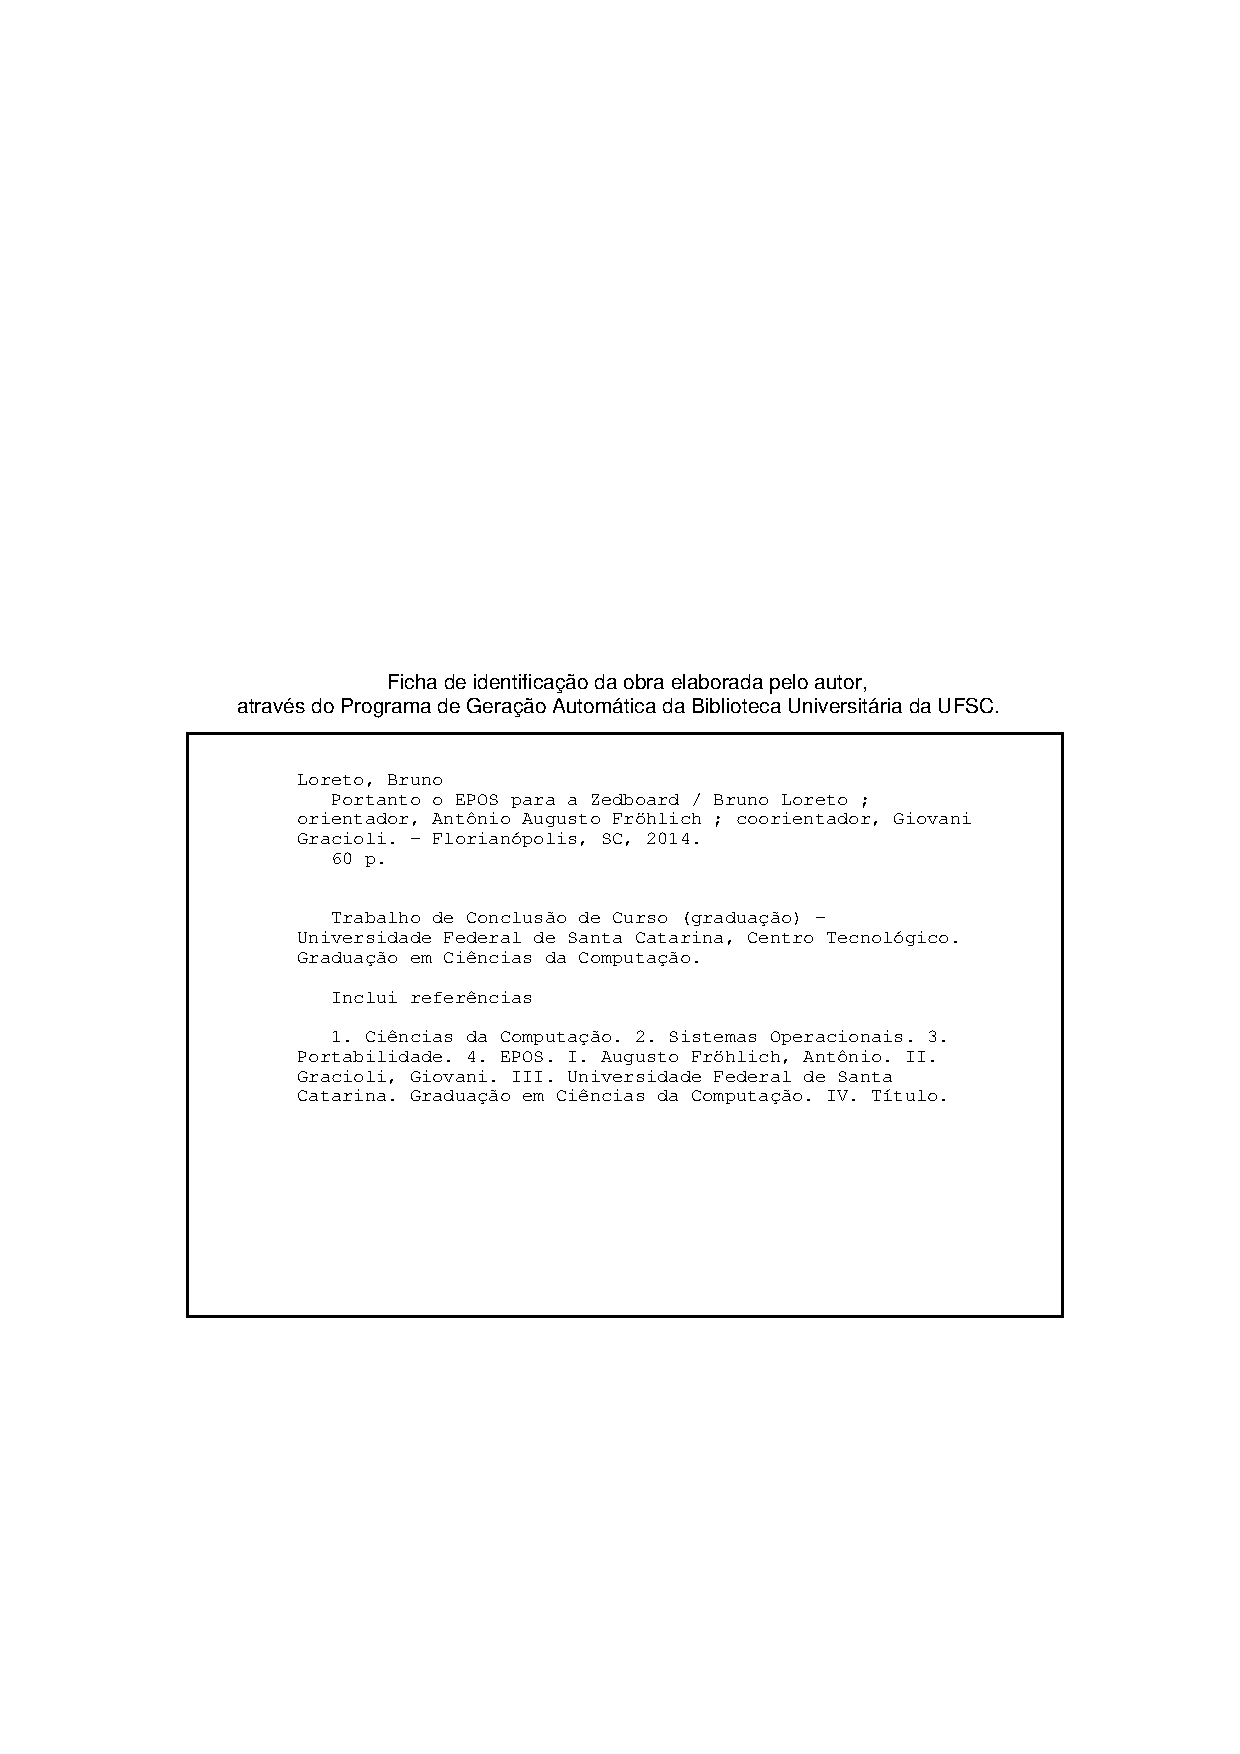
\includepdf[pages={1}]{ufscThesis/ficha.pdf}
\folhaaprovacao
\paginadedicatoria
\paginaagradecimento
\paginaepigrafe
\paginaresumo
\paginaabstract
%\pretextuais % Substitui todos os elementos pre-textuais acima
\listadefiguras % as listas dependem da necessidade do usuário
\listadetabelas 
\listadeabreviaturas
%\listadesimbolos
\sumario

\abreviatura{SoC}{\emph{System-on-Chip}.}
\abreviatura{TCM}{\emph{Tightly Coupled Memory}}
\abreviatura{MMU}{\emph{Memory Management Unit}}
\abreviatura{SP}{\emph{Stack Pointer}}
\abreviatura{PC}{\emph{Program Counter}}
\abreviatura{LR}{\emph{Link Register}}
\abreviatura{CPSR}{\emph{Current Program Status Register}. O registrador que armazena o atual status do processador operante.}
\abreviatura{SPSR}{\emph{Saved Program Status Register}. (Registrador que armazena o valor de CPSR no momento imediatamente anterior ao acontecimento de uma exceção, deste modo o antigo valor de CPSR pode ser restaurado quando a exceção for tratada.}
\abreviatura{CP15}{\emph{System Control Coprocessor}}
\abreviatura{IRQ}{Interrupção normal.}
\abreviatura{FIQ}{\emph{Fast Interrupt}.}
%\abreviatura{SCR}{\emph{ }}
\abreviatura{APSR}{\emph{Application Program Status Register}. Armazena uma cópia do estado das \emph{flags} da unidade lógico-aritimética. Conhecido também como \emph{flag} do código condicional, usados para determinar se uma instrução condicional deve ser executada ou não.}
\abreviatura{GIC}{\emph{Generic Interrupt Controler}}
\abreviatura{rx}{Quando a abreviação rx aparecer, ela estará se referindo genericamente à qualquer um dos 13 primeiros registradores de propósito geral do ARM9 [r0-r12].}
\abreviatura{PPI}{\emph{Private Peripheral Interrupt.}}
\abreviatura{SGI}{\emph{Software Generated Interrupt.}}
\abreviatura{SPI}{\emph{Shared Peripheral Interrupt.}}
\abreviatura{PS}{\emph{Processing system.}}
\abreviatura{PL}{\emph{Programmable Logic.}}
\abreviatura{SMC}{\emph{Static Memory Controller}}
\abreviatura{TSC}{\emph{Time Stamp Counter.}}
\abreviatura{FPGA}{\emph{Field-Programmable Gate Array}. Hardware reconfigurável, o qual têm as suas funcionalidades definidas exclusivamente pelos usuários.}
\abreviatura{PLL}{\emph{Phase-Locked Loop}. É um sistema de controle que gera uma saída cuja fase é relacionada à fase do sinal de entrada. Pode ser usada para estabilizar um sinal e também multiplica-lo.}
\abreviatura{SCU}{\emph{Snoop Control Unit}.}
%--------------------------------------------------------
% Elementos textuais

\chapter{Introdução}

%1) Começar escrevendo sobre a importância de sistemas embarcados;

Sistemas embarcados estão instalados e controlam os mais diversos equipamentos hoje em dia, eles estão mais presentes do que nos damos conta. Conforme eles estão sendo cada vez mais empregados, sua demanda aumenta também, bem como seu poder de processamento. Máquinas que antes utilizavam vários pequenos microcontroladores trabalhando independentemente, hoje podem ser gerenciados com melhor custo-benefício por um sistema de maior desempenho \cite{gio}.%, como há exemplos em carros e aviões.

%2) Citar que alguns desses sistemas demandam maior processamento que só pode ser satisfeito por um hardware dedicado ou por um processador multicore;

Sistemas embarcados estão empregados em tarefas que exigem a manipulação de grande volume de dados (muitas vezes em tempo real), como na área de comunicação e transmissão de dados. O nome ``sistema embarcado'' já foi sinônimo de pequenos microcontroladores dedicados, mas hoje também há grande demanda por sistemas embarcados de alto desempenho. Um meio de obter processamento de alto desempenho à baixo custo é com a implantação de processadores \emph{multicores}.

Aplicações de tempo real necessitam um tempo de resposta previsível, e suas tarefas devem ser executadas com atraso controlável. Um exemplo são os sistemas de airbag automotivo, que necessitam de uma resposta a um estímulo em um determinado intervalo de tempo \cite{nat}. Muitas destas aplicações são feitas diretamente em hardware para se adequar aos requisitos da aplicação (tempo real, gasto energético, etc). Entretanto aplicações feitas diretamente em hardware apresentam problemas em relação à manutenibilidade e possibilidade de atualização \cite{gio}. Estes componentes de hardware poderiam ser centralizados em um sistema embarcado de maior processamento, e alocar tarefas de tempo real para cada uma das funções necessárias ao sistema. Deste modo, a manutenção e custo total do sistema pode ser melhorado, sem necessitar sacrificar as restrições temporais (usando um sistema operacional de tempo real que consiga escalonar o conjunto de tarefas).

Outro exemplo são os quadcópteros. Controlar um quadcóptero não é uma tarefa trivial, há uma miríade de fatores a serem considerados. Um quadcóptero precisa balancear quanto empuxo deve ser aplicado à cada hélice para manter-se no ar e fazer manobras, é necessário também que o sistema seja tolerante à faltas para ser seguro. Em caso de um quadcóptero autônomo, os desafios são ainda maiores. Passa a ser necessário geolocalização, detectar à que distância se está do chão, controle de pouso, etc \cite{leeseshia}.
Não é difícil perceber a grande quantidade de dados a serem processados, e que uma falha em processar estes dados no tempo estimado pode gerar numa falha total do sistema (a queda do quadcóptero, neste caso). Neste exemplo, nota-se como é necessário um sistema operacional previsível, e um hardware capaz de processar rapidamente e paralelamente diversos dados.

%%%%%%%%%%%%%% EPOS %%%%%%%%%%%%%%%%%

%4) Falar da importância de sistemas operacionais de tempo real para sistemas embarcados multicore, principalmente devido ao escalonador;

É natural que estas plataformas de maior desempenho, que consequentemente possuem mais recursos e componentes à serem gerenciados, necessitem de um sistema operacional que se encarregue desta função, e que possam administrar eficientemente estes recursos.
De acordo com um estudo recente \cite{UBM}, a principal razão para usar um sistema operacional é ter garantias de tempo real.

De acordo com este mesmo estudo \cite{UBM}, metade dos projetos de sistemas embarcados usaram mais que um microcontrolador/processador em seu projeto.
Além disto, tem sido comum o uso de FPGAs\footnote{FPGAs podem ser pensadas como um hardware que pode ser programado pelo usuário.} integradas à estes sistemas, onde 31\% dos projetos usaram FPGAs em 2013.
Dentre estas placas, podemos destacar a Zedboard, que é uma plataforma de bom desempenho\footnote{Comparado ao poder de processamento dos demais processadores embarcados.} com um processador \emph{dualcore} de 666 MHz e FPGA.

%5) Citar o EPOS como primeiro RTOS de código aberto a suportar  os escalonadores global, particionado e agrupado;

Uma peça central de um sistema operacional de tempo real é seu escalonador de processos/\emph{threads}. É neste componente que políticas sobre priorização de tarefas são feitas de modo a garantir que cada tarefa seja cumprida dentro de seu prazo.

EPOS, que é um sistema operacional embarcado de tempo real (RTOS\footnote{Real-Time Operating System}) \emph{multithread}, é o o primeiro RTOS de código aberto a suportar os escalonadores de tempo real global, particionado e agrupado \cite{gio}.

%6) Falar que atualmente o EPOS só oferece suporte ao IA32.

Estes fatos demonstram a necessidade de um sistema operacional de tempo real como o EPOS de ter suporte para uma plataforma embarcada multicore. A única arquitetura \emph{multicore} suportada pelo EPOS é a IA32, que não é uma arquitetura que oferece previsibilidade, logo para todos os sistemas embarcados com restrições temporais uma arquitetura multicore com maior previsibilidade torna-se necessário.

O EPOS não possuia suporte para um processador embarcado \emph{multicore}. 
Este trabalho trata de descrever como foi feito o porte
\footnote{Porte é um estrangeirismo da palavra \emph{port}, que, no âmbito da computação, significa o ato de fazer um mesmo programa/sistema/SO funcionar em diferentes ambientes. Por exemplo, fazer um software que antes só funcionava no Linux passar a funcionar em um outro SO (sistema operacional) pode ser considerado um porte. Uma palavra alternativa que poderia ser usada é ``suporte'', entretanto acredito que esta palavra não expresse apropriadamente o que foi feito, já que essa palavra normalmente é associada com um serviço pago de assistência técnica, e o próprio fraseamento do que foi feito se tornaria de mais difícil compreensão e prolixo com esta palavra.}
 deste sistema operacional para a Zedboard, uma plataforma embarcada \emph{multicore}.

\section{Objetivos Gerais}

O objetivo deste trabalho é portar o sistema operacional EPOS para a Zedboard e documentar este processo no presente documento. O porte consiste em adaptar os componentes que, dentro da arquitetura do EPOS, são chamados de mediadores de hardware. Cada mediador precisa ser refeito para cada plataforma\footnote{Aqui chamamos de plataforma qualquer SoC (\emph{System On-Chip}), ou processador. No capítulo \ref{ch:epos} será explicado a diferença entre \emph{machine} e \emph{architecture}, e por enquanto estamos usando a palavra plataforma para nos referenciarmos a estes dois conceitos simultaneamente.}

\section{Objetivos Específicos}
Dos objetivos específicos, pode-se organizá-los da seguinte forma:

\begin{enumerate}
    \item Estudo da arquitetura do EPOS, da arquitetura do ARM Cortex A9 e do Zedboard.
    \item Portes
    \begin{enumerate}
		\item UART
        \item Timers
        \item Controlador de Interrupção
        \item MMU
		\item CPU
		\item Inicialização \emph{multicore}
    \end{enumerate}
%    \item Validações
%    \begin{enumerate}
%        \item Escalonadores em single e multicore
%        \item Threads
%        \item Thread Periódica
%        \item Alarmes
%        \item Cronômetro
%        \item Sincronização
%    \end{enumerate}
    \item Documentação
\end{enumerate}

\section{Organização do Documento}

O restante deste documento é organizado da seguinte forma: No capílo de conceitos básicos serão discutidos de forma suscinta conceitos usados ao longo do trabalho; no capítulo seguinte será dado uma visão geral do hardware escolhido para o porte; no capítulo \ref{ch:epos} será discutido a arquitetura do EPOS, sob um ponto de vista de mais alto nível, sem ainda chegar nos mediadores; e, finalmente, no capítulo \ref{ch:porte}, será explicado o porte em si, comentando as decisões que foram tomadas e como foi organizado o porte\footnote{Organização da memória, sequência de inicialização, etc.}.

\chapter{Conceitos Básicos}

Esta seção tem por objetivo o estabelecimento dos conceitos básicos necessários ao entendimento do restante do trabalho. Não pretende-se aqui fazer uma explicação extensiva e profunda sobre os conceitos expostos, mas sim uma breve introdução, deixando os detalhes para serem procurados pelo leitor nas respectivas referências.


\section{Metaprogramação estática}
Metaprograma é um program que representa e manipula outros programas ou eles próprios \cite{generative}.
Com metaprogramação é possível fazer-se loops (através de recursão), e condicionais (como o \verb+IF+ discutido abaixo), fazendo com que metaprogramas tenham equivalência à máquina de turing \cite{generative}. De fato, a linguagem de metaprogramação do C++ pode ser vista como uma linguagem funcional que tem sua execução em tempo de compilação. Pode-se fazer muitas estruturas metaprogramadas, inclusive listas, árvores e etc, entretanto nesta seção será mostrado apenas o funcionamento básico de um \verb+IF+ metaprogramado, pois este é bastante usado no código do EPOS. Para um maior entendimento sobre o assunto, fica aqui recomendado o livro referenciado \cite{generative}.

A arquitetura do EPOS usa com frequência metaprogramação estática para, em tempo de compilação, selecionar a arquitetura, bem como cada componente que será ou não utilizado. Por exemplo, podemos definir um \verb+if+ estático para selecionar de qual classe a classe Chronometer irá derivar. Primeiramente a definição do \verb+if+:

\begin{lstlisting}
template<bool condition, typename Then, typename Else>
struct IF
{
    typedef Then Result;
};
\end{lstlisting}

Este template, a princípio, nada mais faz do que tomar 3 parâmetros e então criar um tipo chamado \verb+Result+ igual ao segundo parâmetro, contudo, se fizermos uma especialização deste template, ele passa ser útil:

\begin{lstlisting}
template<typename Then, typename Else>
struct IF<false, Then, Else>
{
    typedef Else Result;
};
\end{lstlisting}


Com esta especialização, toda vez que o primeiro parâmetro resolver-se como falso, \verb+Result+ será definido como o terceiro parâmetro. Temos, portanto, um \verb+if+ metaprogramado funcional, agora voltemos ao exemplo do cronômetro.

Suponha que caso a arquitetura não seja multicore, e nos traits o TSC (\emph{time stamp clock}) esteja ativo, então deseja-se que Chronometer derive de TSC\_Chronometer, do contrário de Alarm\_Chronometer.

Isto pode ser feito usando nosso \verb+if+ metaprogramado da seguinte forma:

\begin{lstlisting}
class Chronometer: public
IF<Traits<TSC>::enabled && !Traits<System>::multicore,
TSC_Chronometer, Alarm_Chronometer>::Result
{/*class body*/};
\end{lstlisting}

Deste modo, \verb+Chronomometer+ derivará de \verb+IF::Result+, que será resolvido como TSC\_Chronometer ou Alarm\_Chronometer. Note que esse exemplo também mostra um uso do Traits, onde para descobrir se o TSC está ativo, bastou ler a constante \verb+Traits<TSC>::enabled+, e, para saber se o sistema é multicore, bastou ler \verb+Traits<System>::multicore+. Todo esse processamento causa zero \emph{overhead} em tempo de execução.

\subsection{Traits}

O uso de traits é uma técnica de metaprogramação estática para associar informações aos objetos em tempo de compilação. Por exemplo, uma matriz metaprogramada pode necessitar saber sua dimensão em tempo de compilação. No EPOS, por exemplo, no momento de criação da heap, e de inicialização da MMU, é necessário obter-se informações a respeito do mapeamento de memória do EPOS; estas informações são obtidas através do uso de traits.

Há basicamente 3 maneiras de definirmos traits \cite{generative}:

\begin{description}
\item[Traits como membro da classe:] Forma mais simples de definir-se um trait. Esta técnica basicamente consiste em criar-se constantes e tipos dentro da própria classe que os usa. Esta tecnica é muitas vezes usada sem o programador ter sequer conhecimento que está usando traits.

\item[Classes de traits:] Quando um tipo pode ter muitas características, e pode ser conveniente encapsulá-las numa única classe.

\item[Templates de Traits:] Consiste em definir uma classe de templates para gerenciar uma família de tipos. Esta é a técnica usada no EPOS, e será discutida melhor abaixo.

Nesta técnica, cria-se uma classe genérica, para que esta seja especializada por cada tipo que precisar de traits. Por exemplo, podemos fazer uma classe genérica \verb+number+, para associar informações sobre tipos numéricos, e então especializar esta classe para os diferentes tipos, como \verb+int+, \verb+long+, etc:

\begin{lstlisting}
template<class T>
class number {
public:
	static const bool specialized = false;
	static const unsigned long max = 0;
	static const unsigned long min = 0;
	static const bool sig = false; //Numero com sinal
};
template<>
class number<int> {
public:
	static const bool specialized = true;
	static const unsigned long max = 2147483647;
	static const long min = -2147483648;
	static const bool sig = true;
};
template<>
class number<unsigned long> {
public:
	static const bool specialized = true;
	static const unsigned long max = 4294967296;
	static const long min = 0;
	static const bool sig = false;
};
#include<iostream>
int main(){
	//exemplo de uso
	if(number<int>::specialized)
		std::cout << number<int>::min << std::endl;
	else
		std::cout << "Sem informacoes sobre int\n";
	
	return 0;
}
\end{lstlisting}

Neste exemplo, poderia-se especializar os demais tipos da linguagem C++, assim como adicionar novos atributos à estas especializações. Note que deste modo é possível centralizar num único arquivo várias características de vários tipos distintos, de forma organizada, de fácil manutenção e edição. No EPOS, os mais diversos componentes do SO podem ser configurados facilmente através dos traits; veja a seção \ref{sec:traits} para mais detalhes.


\end{description}

%%%%
\section{Registradores Mapeados em Memória}
Uma maneira usada para se comunicar, configurar e ler o estado de um dado componente de hardware é através da leitura e/ou escrita em registradores mapeados em memória. Um registrador mapeado em memória basicamente é uma região fixa da memória, onde uma escrita naquela posição indica uma escrita no registrador lá mapeado.
Exemplificando, a UART da Zedboard possui um registrador chamado rcvr\_timeout\_reg0, responsável por indicar quantos ciclos\footnote{Na realidade é o número de baud\_samples que se passaram.} a UART deve esperar um novo caractere chegar antes de emitir uma interrupção de \emph{timeout}. Este registrador está mapeado na posição de memória 0xE000001C para a UART0. Portanto, para configurar que o número de ciclos esperado seja de 20, basta escrever este número naquela posição. Uma maneira de fazer esta escrita, por exemplo, em C/C++, é: \verb+*((unsigned long*)0xE000001C) = 20;+.

%%%%
\section{Orientação a Objetos}
Programação orientada a objetos é um método de implementação no qual programas são organizados como coleções cooperantes de objetos, cada qual representa uma instância de alguma classe, sendo que estas classes são todas membros de uma hierarquia de classes unidas por relações de herança \cite{OOAD}.

%%%%
\section{Sistema Operacional}
Tanenbaum define sistemas operacionais sob duas perspectivas \cite{tanenbaum}:

\textbf{SO como uma máquina extendida:}
Programar ao nível de linguagem de máquina pode ser um tanto desastroso e desnecessariamente complicado. Por exemplo, na arquitetura PD765, o controlador de um disquete possui 16 comandos de controle, sendo os mais básicos os comandos WRITE e READ. Cada um destes comandos requerem 13 parâmetros, codificados em 9 bytes, parâmetros estes que específicam o endereço do bloco a ser lido, número de setores por trilha, modo de gravação desejada, etc.

Certamente um programador não quer ter que lidar com esse tipo de detalhe, e no lugar ele gostaria apenas de ter uma simples abstração de arquivos que podem ser abertos, editados, salvos e fechados.
O programa que procura esconder estes detalhes sórdidos é o sistema operacional, que procura abstrair o gerenciamento de arquivos, assim como detalhes sobre tratamento de interrupções, timers, gerenciamento de memória e qualquer outro detalhe de baixo nível, fazendo assim o programador ter a ilusão de estar interagindo com uma máquina mais simples e de mais alto nível.

\textbf{SO como um gerenciador de recursos:}
Diferentes processos competem entre si por utilizar os recursos do sistema. Estes processos precisam compartilhar entre si memória, tempo na CPU, dispositivos de entrada e saída, impressoras, etc. O programa responsável por conciliar as necessidades de cada processo, gerenciando os recursos da máquina de forma organizada e que atenda à todas as requisições por eles é, também, o sistema operacional.

\subsection{Processo}
Um processo basicamente é um programa \emph{em execução}, incluindo o seu \emph{program counter}, registradores e variáveis \cite{tanenbaum}. Cada processo possui um espaço de endereçamento próprio e individual, estando protegidos (e impedidos) de acessarem a porção de memória alocada para os demais processos. Cada processo executa na CPU por um certo intervalo de tempo, e então, caso não tenha terminado sua execução, esta é interrompida pelo escalonador de processos (veja seção \ref{escalonador}) para que a CPU possa ser usada por outro processo.

\subsection{Thread}
Todo processo está rodando pelo menos uma thread, e um conjunto de threads pode pertencer ao mesmo processo (toda thread pertence à algum processo). Cada thread pode executar independentemente, de forma pseudoparalela
\footnote{Em uma arquitetura de processador com apenas um núcleo, todos os processos e threads executam na realidade sequencialmente, entretanto parecem ser executadas paralelamente devido à pequena fatia de tempo que cada processo/thread possui para executar, por isto chamamos isto de pseudoparalelismo. Mesmo em arquiteturas de multiplos núcleos o paralelismo ``verdadeiro'' ainda não acontece com frequência, já que basta existirem mais processos/threads do que o número de núcleos para que estes tenham que ser sequenciados.}
, entretanto cada thread compartilha do espaço de endereçamento do processo ao qual pertencem. Cada thread possui seu próprio contexto, isto é, o estado de seus registradores (incluindo o \emph{program counter}, pilha e etc).
A vantagem de threads sobre processos é que a comunicação entre threads de um mesmo processo é muito mais rápida que a comunicação intraprocessos, e criar uma thread é mais rápido que criar um processo também.

\subsection{Escalonador}
\label{escalonador}

Um escalonador de processos (ou threads) é responsável por garantir que cada processo/thread consiga executar por algum determinado tempo na CPU. Existem diversos algoritmos de escalonamento, vários deles tendo sido implementados no EPOS. De acordo com Tanenbaum, há cinco dimensões que um escalonador deve levar em consideração em sua política de escalonamento \cite{tanenbaum}:

\begin{enumerate}
\item \textbf{Justiça (Fairness):} Assegurar que cada processo consiga executar por um tempo justo na CPU.
\item \textbf{Eficiência:} Tentar manter a CPU ocupada pela maior parte do tempo.
\item \textbf{Tempo de Resposta:} Minimizar o tempo de reposta para aplicações interativas.
\item \textbf{Turnaround:} Minimizar o tempo que processos \emph{batch} precisam esperar para executar.
\item \textbf{Vazão (throughput):} Maximizar a quantidade de tarefas realizadas por unidade de tempo.
\end{enumerate}

Claro que alguns destes itens são contraditórios entre si, por isto a escolha de um algoritmo de escalonamento depende da aplicação e carga de trabalho que o sistema pretende lidar.

% TODO Escalonadores de tempo real

\section{Sistema Embarcado}

É cada vez mais difícil definir o que é um sistema embarcado. Hoje sistemas embarcados estão em todos os lugares, eles acionam motores, freios, cintos de segurança, airbags, sistemas de audio em um carro. Eles codificam digitalmente voz e constroem sinais de radio e enviam eles de um celular para uma estação. Eles controlam microondas, ar-condicionados, semáforos, etc.

Existem sistemas embarcados dos mais diversos tamanhos e capacidades, desde aqueles com um \emph{clock} de poucos KHz, até processadores com GHz. Podemos dizer o que \emph{não} é um sistema embarcado: Notebooks, desktop, servidores e supercomputadores. É arriscar incorrer em erro tentar dar uma definição mais precisa \cite{leeseshia}.

\section{Sistemas de Tempo Real}

Sistemas de tempo real são definidos como aqueles sistemas nos quais a corretude geral do sistema depende tanto da corretude funcional (produzir o resultado correto) quanto a corretude temporal (produzir o resultado dentro do tempo máximo de tolerância). A corretude temporal é pelo menos tão importante quanto a corretude funcional \cite{realtime}. Ou seja, cada tarefa não somente deve produzir o resultado correto, mas também produzi-lo dentro de um intervalo de tempo predeterminado. Note que nem todos os sistemas de tempo real são sistemas embarcados, apesar de existir uma grande área em comum \footnote{Um sistema que oferece um serviço de \emph{streaming} de vídeo, por exemplo, é um sistema \emph{soft real-time}, mas não necessariamente embarcado.}\cite{realtime}. Os sistemas de tempo real podem ser classificados em duas categorias:

\begin{description}
	\item[Hard real-time] Nesta categoria, as tarefas dos sistemas devem necessariamente ser concluídas dentro do prazo, do contrário a resposta da tarefa já não faz mais sentido, e esta perda de prazo pode causar uma falha catastrófica do sistema, possivelmente causando grande prejuízo e até mesmo por vidas humanas em risco.
	\item[Soft real-time] Estes sistemas também precisam que suas tarefas sejam concluídas dentro do prazo, entretanto há certa tolerancia à atrasos, e no lugar de causar uma falha no sistema, a sucessiva perda de prazos costuma causar degradação do desempenho do sistema.
\end{description}

Exemplos de sistemas \emph{hard real-time} são vários. Imagine um sistema de detecção de mísseis, e que procura abater estes mísseis atirando neles. Fica claro que o tempo entre a detecção e a ação (atirar no míssil) está limitada à uma certa janela de tempo, e que a perda dessa janela de tempo pode resultar em ser acertado por um míssil \cite{realtime}.

Por outro lado, podemos imaginar também um reprodutor de vídeo. Cada \emph{frame} deve ser decodificado dentro de certa janela de tempo, do contrário aquele quadro pode não mais fazer sentido. Entretanto estes sistemas são tolerantes à perda de alguns quadros, portanto uma demora na codificação resulta numa degradação no desempenho (menor taxa de quadros por segundo), mas não evitam do vídeo não ser mais reproduzível. Este é um exemplo de sistema \emph{soft real-time}.

\section{Exceções e Interrupções}
Na terminologia adotada neste trabalho, uma exceção é um evento inesperado, que interrompe o processando normal do programa, fazendo o registrador PC apontar para uma região específica de memória, onde o tratador daquela exceção reside. Estas exceções incluem erros de permissão de leitura de certa parte da memória, tentativa de execução de uma instrução inválida (mal formada), etc.

Interrupções são bastante semelhantes à exceções. Elas param o fluxo normal de processamento, e também fazem com que a próxima instrução executada seja aquela numa região pré determinada da memória onde está o tratador daquela interrupção. A diferença esta no fato de interrupções poderem ser mascaradas, desativadas e gerenciadas pelo controlador de interrupção, enquanto não há controle sobre a execução das exceções (não são passíveis de desativação). Outra diferença, mais conceitual, é o fato que interrupções em geral são desejáveis e frequentemente necessárias para o funcionamento do sistema, enquanto exceções ocorrem apenas quando algo imprevisto é executado (como a execução de uma área de memória que não possui instruções executáveis).

A princípio, do ponto de vista do processador, uma interrução não tem muita diferença de uma exceção, por isto que no primeiro nível a interrupção é pré processada por um tratador de exceções, para então ser encaminhada para um tratador de interrupções (como mostra a figura \ref{fig:exception_handling}).


\section{MMU} %http://epos.lisha.ufsc.br/EPOS+User+Guide#MMU
A MMU (\emph{Memory Managemed Unit}) é um componente responsável por gerenciar a memória de um sistema. É este componente o responsável por traduzir o endereçamento lógico (memória virtual) em endereçamento físico (memória física). Uma das principais vantagens de seu uso é a possibilidade de proteção de memória (entre processos e SO) e facilitação da escrita de aplicativos, pois estes não precisam levar em consideração o mapa de memória do SO.

\section{UART}
A UART (Universal Asynchronous Receiver/Transmitter) é um componente que trata da saída e entrada serial do sistema, portanto sendo o componente responsável por transmitir e receber caracteres, sendo necessário para impressão em tela, o que pode ser feito por via USB (usado principalmente para depuração do código). As duas principais funções na classe da UART dentro do EPOS são justamente a put e get, para impressão e leitura de caractere, respectivamente. O Zynq possui duas UARTs.


\section{\emph{Timer}}

\emph{Timer} é um componente de hardware que pode ser configurado para contar um certo número de ciclos. Ao fim da contagem o \emph{timer} emite uma interrupção, que então o processador pode tratar. Este componente é fundamental para um escalonador de processos e \emph{threads}.


\section{Ambiente de Desenvolvimento}

O ambiente de desenvolvimento usado para o porte foi o qemu para ARM (\verb+qemu-system-arm+) modificado pela Xilinx, para executar o EPOS num ambiente virtualizado (emulado), pois assim pode-se usar ferramentas como o GDB para a depuração do código de forma rápida. O uso do GDB foi fundamental para o desenvolvimento, já que com ele era possível imprimir o valor de cada registrador em um dado ponto da execução, verificar a memória, executar instruções específicas e etc. Para compilar o EPOS foi usado \emph{cross-compilers} para ARM. As flags usadas para criar um ambiente de depuração com o qemu e o GDB foram as seguintes (com cada comando feito em um terminal diferente):
%\hspace*{-1.0cm}\vbox{
\begin{verbatim}
./qemu-system-arm -kern-dtb ./xilinx_zynq.dtb \
    -no-reboot -nographic -smp 2 -machine xilinx-zynq-a9 \
    -cpu cortex-a9 -kernel img/panda_app -m 512 \
    -fda img/panda_app.img

arm-none-eabi-gdb -ex "target remote :1234"
\end{verbatim}
%}

O hardware real também estava disponível, e foi usado quando o qemu não produzia resultados confiáveis. Com o hardware real, para a depuração do código foi usado o JTAG.
Para carregar a imagem do SO na placa, foi usada a ferramenta da Xilinx \verb-xmd-, sendo que esta ferramenta trata de fazer o processador apontar para o ponto de entrada da imagem carregada, de tal modo que é possível conectar o GDB através da porta aberta pelo \verb+xmd+, e então executar através do GDB.

\chapter{Hardware-alvo}

%source: http://www.zedboard.org/product/zedboard
% http://www.zedboard.org/sites/default/files/documentations/ZedBoard_HW_UG_v2_2.pdf
Zedboard é uma plataforma de desenvolvimento que suporta uma grande variedade de aplicações, visto que ela possui uma boa gama de interfaces e funções para habilitar isto. É dedicada à prototipação e \emph{proof-of-concept}. Em seu interior ela possui um Xilinx Zynq 7000 (Z-7020), que é a arquitetura alvo deste porte. A figura \ref{fig:zed} mostra como é a placa fisicamente.

O ZYNQ-7000 SOC XC7Z020-CLG484-1 conta com o processador Dual ARM Cortex-A9 MPCore. O Zynq possui 4 graduações de velocidade de \emph{clock}, a comercial (graduação -1), industrial (graduação -1 a -2), estendida (-2 a -3) e expandida (-1), sendo a graduação -1 a menor velocidade, e a -3 a maior \cite{product_table}.

De acordo com a especificação da Zedboard \cite{zedboard}, o \emph{clock} máximo do processador é de 667MHZ, portanto, tendo como referência a tabela de dados do Zynq-7000 \cite[p.~13]{data_sheet}, chegamos à conclusão que a graduação de velocidade do Zynq usado na Zedboard é de -1 (comercial), esta informação se tornará útil mais à frente.

Há disponível 512MB de RAM DDR3, e um SD card de 4GB. A Zedboard suporta conexão com JTAG, saída serial (USB UART) e conexão com a internet \cite{xilinx}.

A família Zynq 7000 disponibiliza para o desenvolvedor FPGAs, tornando esta plataforma mais configurável e flexível \cite[p.~26]{ug585}. A PS dessa família é a mesma para cada dispositivo onde ela se encontra, entretanto a PL e recursos de entrada e saída variam entre diferentes dispositivos. 


\begin{figure}[ht!]
	\label{fig:zed}
    \centering
    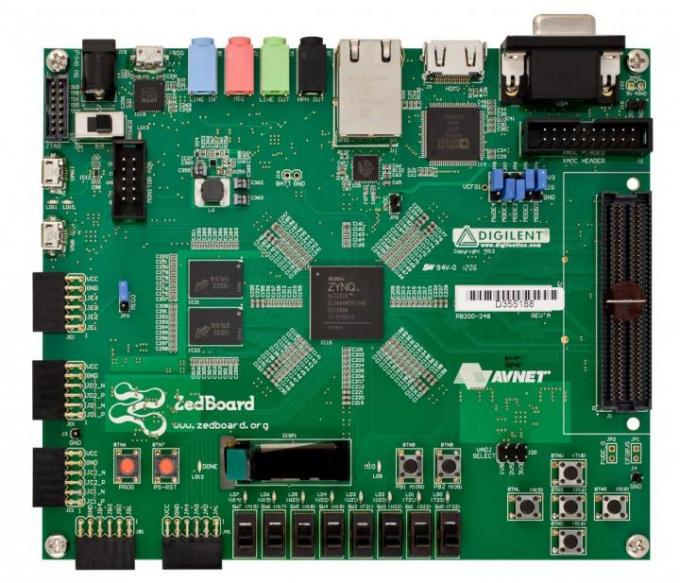
\includegraphics[width=8cm]{figuras/zedboard}
    \caption{Zedboard visto de cima.}
\end{figure}

\section{Arquitetura do Zynq 7000}
Como já citado, o Zynq 7000 possui um processador \emph{dual core} Cortex A9, cada core possui sua própria MMU e memória cache L1 (instruções e dados) privada.

%layout de memoria
\section{OCM} O \emph{On-chip Memory} é uma pequena memória de 256KB de RAM que fica próxima ao processador, e portanto tem um acesso mais rápido. O OCM pode ser mapeado nos primeiros 256KB do espaço de endereçamento, ou nos últimos 256KB do espaço de endereçamento \cite{ug585}.


\section{Modos de Operação}
\label{sec:operating_modes}
A arquitetura ARMv7 conta com 9 modos de operação (7 por padrão, mais 2 com extensões habilidadas), sendo que o único modo não privilegiado é o modo de usuário, os demais modos padrão possuem o mesmo privilégio dentro do sistema\footnote{O modo hipervisor possui certas funções que os demais modos não oferecem, mas no que diz respeito à acesso a memória e execução de instruções, ainda é o mesmo privilégio}. A principal diferença entre um modo e outro é que cada modo conta com um certo subconjunto privado de registradores banqueados, visiveis somente no modo em vigência, como ilustra a imagem \ref{fig:banked}. A tabela \ref{tab:processormode} ilustra quais são os modos de operação disponíveis \cite[p.~1139]{armarm}.
O campo ``Codificação'' é usado no registrador CPSR para se verificar ou modificar o modo de operação vigente.

\begin{table}[ht]
\centering
\begin{tabular}{ccc}
\hline\hline                        %inserts double horizontal lines
Modo do processador  & Codificação & Implementado?\\ [0.5ex] % inserts table 
%heading
\hline                  % inserts single horizontal line
User & 10000 & Sempre \\
FIQ & 10001 & Sempre \\
IRQ & 10010 & Sempre \\
Supervisor & 10011 & Sempre\\
Monitor & 10110 & Com extensões de segurança.\\
Abort & 10111 & Sempre\\
Hyp & 11010 & Com extensões de virtualização.\\
Undefined & 11011 & Sempre\\
System & 11111 & Sempre\\[1ex]
\hline %inserts single line
\end{tabular}
\caption{Modos do processador. Codificação corresponde aos bits CPSR[4:0].}
\label{tab:processormode} % is used to refer this table in the text
\end{table}

\textbf{Modo Usuário:} Modo não-privilegiado de execução. Neste modo somente é possível de se fazer acesso não privilegiado aos recursos do hardware (não prodendo acessar as áreas protegidas). Não é possível de se mudar para outro modo de operação quando neste, a não ser por eventos externos como interrupções.

\textbf{Modo Sistema:} Modo privilegiado de execução. Este modo usa os mesmos registradores que o modo usuário e nenhuma exceção leva a este modo. Somente é possível de se entrar nesse modo alterando os bits do registrador de status do sistema (CPSR); é necessário já estar em algum modo privilegiado para tal operação.

\textbf{Modo Supervisor:} É o modo padrão para no qual processador entra quando uma exceção do tipo \emph{Supervisor Call} é recebida.
Para gerar um \emph{Supervisor Call}, usa-se a instrução \verb+svc+. O processador entra neste modo ao se resetar.

\textbf{Modo Abort:} Modo que o processador entra quando recebe uma interrupção do tipo \emph{prefetch abort} ou \emph{data abort}.

\textbf{Modo Indefinido:} Modo que o processador entra quando se tenta executar uma instrução não definida.

\textbf{Modo FIQ:} Modo que o processador entra quando recebe uma interrupção FIQ.

\textbf{Modo IRQ:} Modo que o processador entra quando recebe uma interrupção IRQ.

\textbf{Modo Hipervisor:} Este modo possui alguns privilégios a mais que os demais modos, mas somente existe quando as extensões de virtualização estão ativas (fora do escopo deste trabalho).

\textbf{Modo Monitor:} Modo que o processador entra quando recebe uma interrupção \emph{Secure Monitor Call}, \verb+SMC+. Este modo está fora do escopo do trabalho.


\begin{figure}[ht!]
	\centerline{
    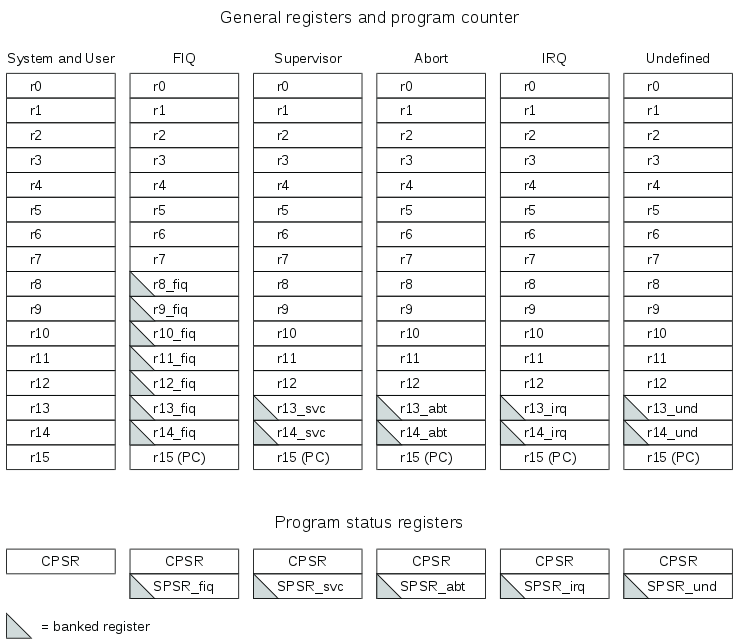
\includegraphics[width=12cm]{figuras/banked_registers}
	}
    \caption{Registradores banqueados.}
	\label{fig:banked}
\end{figure}



\section{GIC}
O GIC (\emph{Generic Interrupt Controller}) é um componente que centraliza e administra todas as interrupções do sistema, ativando, desativando, mascarando e priorizando as fontes de interrupção.


\section{Tipos de Interrupção} %ug585 p. 192
\label{sec:interrupt}
\textbf{Interrupção Gerada por Software: }
Cada CPU pode se interromper, interromper outra CPU, ou ambas CPUs usando SGIs (\emph{Software Generated Interrupts}). Existem 16 interrupções geradas por software, que podem ser geradas escrevendo o número da interrupção ([0-15]), junto com o número da CPU alvo no registrador ICDSGIR. Esta escrita ocorre dentro do barramento privado da própria CPU. Cada CPU possui seu próprio conjunto privado de registradores de SGIs para gerarem uma (ou mais) das 16 SGIs possíveis \cite[p.~216]{ug585.1.7}. É possível limpar uma interrupção lendo o registrador ICCIAR (\emph{Interrupt Acknowledge}) ou escrevendo 1 nos bits correspondentes do registrador ICDICPR (\emph{Interrupt Clear-Pending}).
\\\\
\textbf{Interrupções de Periféricos Privados da CPU: }
\\\\
\textbf{Interrupções de Periféricos Compartilhados: }
Existem cerca de 60 interrupções de diversos modulos que podem ser roteadas para um ou ambos processadores, ou para a lógica programável. O GIC é responsável por administrar estas interrupções. Além das interrupções IRQ, há também interrupções do tipo FIQ e geradas por software.

\textbf{FIQ \emph{Fast Interrupt}:} O modo FIQ possui um número maior de registradores banqueados que os demais modos (R8 até R13, além do SP, LR e SPSR), fazendo com que não seja necessário fazer troca de contexto. FIQs também tem mais alta prioridade que qualquer IRQ, pontanto este tipo de interrupção é apropriado para aplicações de tempo real de usuário único. Se multiplas aplicações tempo real usarem FIQ, pode haver conflitos de interesse que podem fazer um processo perder um \emph{deadline} \cite[p.~66]{armarm}.

\textbf{Interrupção de Software: } Existe uma instrução no assembly do ARMv7 que permite que seja feita uma interrupção de software (\verb+swi+). Esta instrução pode ser acompanhada de um número de 8 bits. Esta interrupção leva ao modo supervisor.

%FIQ mode is designed for efficient use by a single owner, using R8_fiq - R13_fiq as global variables. 
%In addition, unlike IRQs, FIQs are not disabled by other exceptions (apart from reset), making them 
%the preferred type for real time interrupts, when other exceptions are being used routinely, such as 
%virtual memory or instruction emulation. IRQs may be disabled for unacceptably long periods of time 
%while these needs are being serviced.
%However, if more than one real-time interrupt source is required, there is a conflict of interest. The 
%new mechanism allows multiple FIQ sources and minimizes the period with FIQs disabled, greatly 
%reducing the interrupt latency penalty. The FIQ mode registers can be allocated to the highest priority 
%FIQ as a single owner
%ARM ARM p. 66.

A Zedboard possui também as seguintes exceções\footnote{Em conceitos básicos está colocada a diferença entre interrupções e exceções}:

\textbf{Instrução não definida (\emph{Undefined Instruction}):} 
Há duas situações que geram esta interrupção: Quando se executa instruções de coprocessador que não são reconhecidas por este, ou quando se executa instruções que não possuem significado para o processador \cite[p.~36]{armarm}. Normalmente este tipo de interrupção acontecerá quando o processador estiver lendo e tentando executar lixo de memória.


\textbf{\emph{Prefetch Abort: }} Interrupção que leva ao modo \emph{Abort}. Este tipo de interrupção é sinalizado pelo sistema de memória (MMU). Através da MMU, é possível de se marcar certas regiões de memória como não executáveis; isto é importante de se fazer em regiões de memória que possuem dados sensíveis, de modo que quando o processador tentar ler aquela área para executar num futuro próximo, a MMU envia um sinal invalidando aquilo que foi lido. Quando o processador tenta executar uma instrução que tenha sido anteriormente invalidada, uma interrupção do tipo \emph{prefetch} ocorre \cite[p.~58]{armarm}. Note que é possível do processador ler aquela região para executar em seguida, mas ainda não gerar esta interrupção; isto ocorre quando o fluxo é desviado antes da tentativa de executar aquela instrução (por um \emph{branch} por exemplo).

\textbf{\emph{Data Abort:}} Assim como a \emph{prefetch abort}, esta interrupção também leva ao modo \emph{Abort} (e somente estas duas interrupções). Este tipo de interrupção pode acontecer quando uma instrução tenta acessar uma região de memória que o modo atual de execução não tenha permissão para acessar. Acesso a regiões de memória virtual não mapeadas pela MMU também geram esta interrupção.


%Source: http://infocenter.arm.com/help/index.jsp?topic=/com.arm.doc.dui0068b/BABFCEEG.html


\section{\emph{Timers}}
Cada um dos \emph{cores} possui um \emph{timer} privado de 32 bits e ambos \emph{cores} compartilham um \emph{timer} global de 64 bits. Estes \emph{timers} trabalham numa frequência sempre igual à metade da frequência da CPU.
No nível de sistema (\emph{sistem-level (PS)}), há dois grupos independentes de \emph{timers}, cada grupo com 3 \emph{timers}.




\section{\emph{Clocks}}

%30 <= PS_CLK <= 60MHZ
O \emph{clock} principal do sistema, chamado aqui de PS\_CLK (\emph{Processing System Clock}), é responsável por alimentar as 3 PLLs\footnote{\emph{Phase-Locked Loop}. É um sistema de controle que gera uma saída cuja fase é relacionada à fase do sinal de entrada. Pode ser usada para estabilizar um sinal e também multiplica-lo.} do sistema, sendo cada uma dessas PLLs responsável por uma parte diferente do sistema \cite[p.~622]{ug585}. O PS\_CLK é um \emph{clock} de baixa frequência, ficando entre 30 a 60 MHz (PS\_CLK é igual a 33.33 MHz no caso da Zedboard \cite[p.~19]{zed_manual}), sendo este multiplicado por cada uma das 3 PLLs para que o sistema funcione com velocidades maiores\footnote{Este clock pode ser multiplicado por um número de 1 a 127, e é multiplicado por 26 por padrão.}. As 3 PLLs são:

\begin{itemize}
	\item \textbf{I/O PLL:} Responsável por produzir o sinal de \emph{clock} para os dispositivos de entrada e saída.
	\item \textbf{DDR PLL:} Responsável por produzir o sinal de \emph{clock} para as memórias da plataforma.
	\item \textbf{ARM PLL:} Responsável por produzir o sinal de \emph{clock} do restante do sistema, incluindo os processadores.
\end{itemize}

A FPGA da Zedboard possui um \emph{clock} próprio e exclusivo. A figura \ref{fig:clocks} ilustra como estão dispostos estes \emph{clocks}.

\begin{figure}[ht!]
	\centerline{
    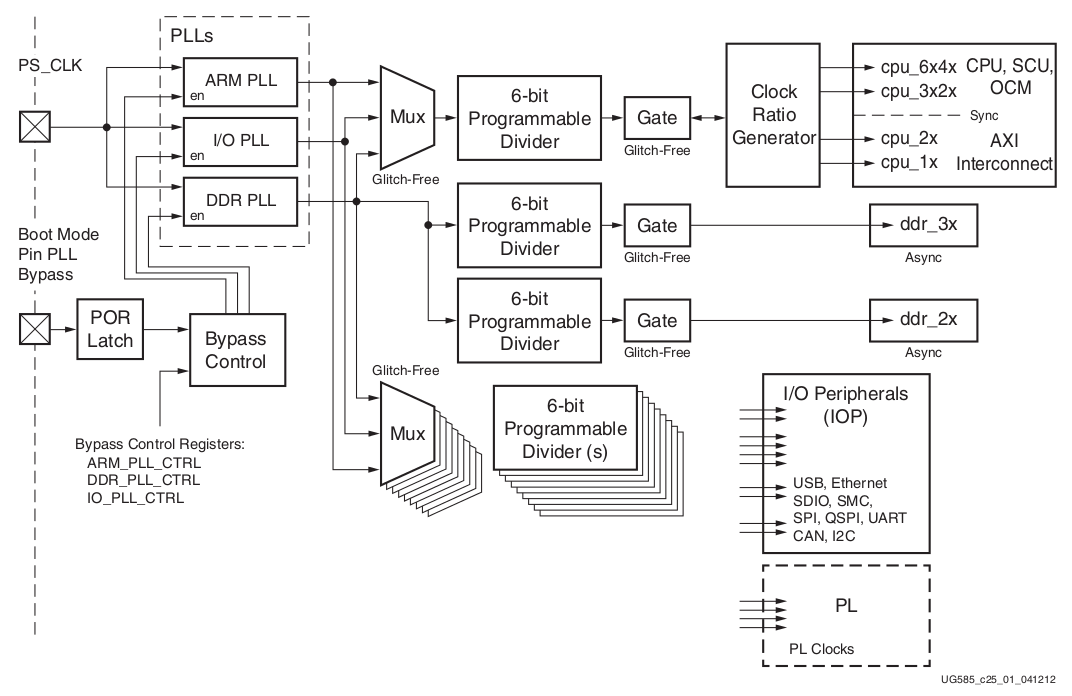
\includegraphics[width=13cm]{figuras/clocks}
	}
    \caption{Diagrama de blocos dos \emph{clocks} disponíveis no Zynq. Note os \emph{clocks} da tabela \ref{tab:clocks} no canto superior direito da imagem.}
	\label{fig:clocks}
\end{figure}

A Zedboard pode operar em dois modos (ou velocidades), denominados pela pela razão 6:3:2:1 e 4:2:2:1, abreviados como 6:2:1 e 4:2:1. Para alternar entre estes dois modos de velocidade, basta escrever 1 ou 0 no registrador CLK\_621\_TRUE. Estes números indicam quantas vezes cada \emph{clock} multiplica o \emph{clock} de base CPU\_1x, sendo este CPU\_1x um \emph{clock} derivado da ARM PLL, dividido por algum fator (configurável).

Há 4 \emph{clocks} independentes, chamados de CPU\_6x4x, CPU\_3x2x, CPU\_2x e CPU\_1x. Esta nomenclatura dos \emph{clocks} indica o fator pelo qual o CPU\_1x é multiplicado em cada modo.
O primeiro número do nome indica o fator multiplicativo daquele \emph{clock} no modo 6:2:1, e o segundo número indica o fator multiplicativo no modo 4:2:1.
Por exemplo, no modo \textbf{6}:2:1, o CPU\_\textbf{6x}4x multiplica o CPU\_1x 6 vezes, e no modo \textbf{4}:2:1, o CPU\_6x\textbf{4x} multiplica o CPU\_1x 4 vezes. A tabela \ref{tab:clocks} ilustra a velocidade de cada \emph{clock} em cada um dos dois modos.

\begin{table}[ht]
	\centering
	\begin{tabular}{ccc}
		\hline\hline
		Nomenclatura & \emph{Clock Ratio Mode} & Máxima frequência da CPU\\[0.5ex]
		\hline
		CPU\_6x4x & \multirow{4}{*}{6:3:2:1} & 667 MHZ\\
		CPU\_3x2x &                          & 333 MHZ\\
		CPU\_2x   &                          & 222 MHZ\\
		CPU\_1x   &                          & 111 MHZ\\
		\hline
		CPU\_6x4x & \multirow{4}{*}{4:2:2:1} & 533 MHZ\\
		CPU\_3x2x &                          & 267 MHZ\\
		CPU\_2x   &                          & 267 MHZ\\
		CPU\_1x   &                          & 133 MHZ\\[1ex]
		\hline
	\end{tabular}
	\caption{Máximas frequências possíveis para cada configuração de \emph{clock}. Para uma lista mais completa (com as diferentes graduações de \emph{clock}), veja \cite[p.~13]{data_sheet}.}
	\label{tab:clocks}
\end{table}

%\begin{figure}[ht!]
%    \centering
%    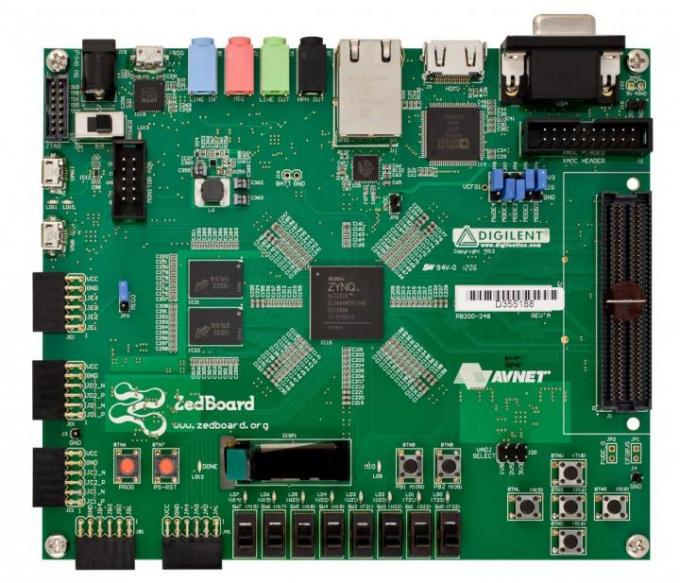
\includegraphics[width=8cm]{figuras/zedboard}
%	\caption{Arquitetura do Zynq 7000.}
%\end{figure}







%Falar que a MMU tem dois níveis, tamanho dela, etc...



%%%%%%%%
%		Get image from ug585 v1.7 p.79!
%%%%%%%%



%conceitos básicos deviam ser mais abstratos, e não falar a respeito de características da placa/processador físico.

\chapter{EPOS}

%alarm's diagram
%alarm's queue

%scheduling

%Processo de inicialização do epos (crt, inits, etc).
%explicar crts... (good luck on that my boy).
%falar talvez do estilo do código (_asdf é private, etc).
%epos mote

%cite some works that used EPOS (specially giovani's).


%source: http://epos.lisha.ufsc.br/EPOS+User+Guide
EPOS (Embedded Parallel Operating System) é um sistema operacional orientado a aplicação, cujo design chama-se ADESD (\emph{Application-Driven Embedded System Design Method}), proposto por Fröhlich \cite{guto_thesis}. A ideia central do EPOS é prover um sistema operacional mínimo, de modo a minimizar o \emph{overhead} da existência de um sistema operacional, deixando o processador livre para executar a aplicação do desenvolvedor \cite{epos_user_guide}.

Como o objetivo é criar um ambiente em que o desenvolvedor possa rapidamente produzir suas aplicações, EPOS provê vários utilitários comumente usados em aplicações, como filas, listas, tabelas de hashs, vetores, semáforos, OStream (para imprimir na tela), números aleatórios, cálculo de CRC e etc. Além destes utilitários, EPOS também provê uma série de componentes como threads, alarmes, cronometros, \emph{heaps} e meios para acessar a rede (internet).

\section{Arquitetura do EPOS}


\textbf{Linguagem e paradigma:} O EPOS é escrito em C++, e não em C, como é tradicionalmente feito. Como paradigma, é usado orientação à objetos, então cada componente do EPOS está encapsulado por uma classe (como a heap, timer, thread, etc). No EPOS também é muito usado conceitos como herança e metaprogramação estática (que será abordado mais a frente).

\textbf{Mediadores de Hardware:} Dentro da arquitetura do EPOS há o conceito de mediadores de hardware, que são os componentes (ou classes) dependentes de plataforma. Idealmente, as únicas classes que precisam ser modificadas e/ou reimplementadas são os mediadores. Há mediadores específicos da placa, como por exemplo Pandaboard, Zedboard e etc; abstraídos sob o nome de \emph{machine} e mediadores específicos de um processador, abstraídos sob o nome de \emph{architecture}. No código do EPOS, estes mediadores encontram-se nas pastas \emph{mach} e \emph{arch}.
% Fonte: Hardware Mediators: A Portability Artifact for Component-based Systems
% HAL vs Virtualização vs Mediadores

Mediadores de hardware são uma alternativa ao tradicional uso de VMs\footnote{Virtual Machines.} e de HAL\footnote{Hardware Abstraction Layer}, proposta por Fröhlich em seu trabalho \emph{Application-Oriented System Design} \cite{guto_thesis}. O problema do uso de VMs é o seu \emph{overhead} causado devido à tradução das operações da VM em código nativo. Já o uso de um HAL incorre no problema da manutenibilidade e dificuldade de adapção à novas arquiteturas muito distintas entre si \cite{hw_mediators}. O HAL não conseguiu passar pela ``prova do tempo'', e já está sendo considerado obsoleto por distribuições GNU/Linux populares, como o 
Ubuntu\footnote{\url{http://www.linux-magazine.com/Online/News/Ubuntu-10.04-Alpha-2-Removes-HAL}}, sendo chamado de ``uma grande não-manutenível bagunça monolítica''\footnote{\url{https://wiki.ubuntu.com/Halsectomy}}.

%\textbf{Traits:} Traits são classes onde é possível configurar certos componentes do EPOS em tempo de compilação. Lá é possível, por exemplo, definir o tamanho da \emph{stack} e \emph{heap} do sistema, a sua frequência de \emph{clock} bem como ativar ou desativar certas funções do sistema. Esta classe normalmente precisa ser alterada em um porte, mesmo ela não sendo um mediador de hardware, pois eles usam as configurações descritas nos traits.

\textbf{Interface Infladas: } Um conceito importante da arquitetura do EPOS é a Interface Inflada. %http://www.inf.ufsc.br/~guto/publications/aoos.pdf
Em sistemas orientados a aplicação, famílias de abstrações são frequentemente tratadas como entidades únicas, algo que pode ser vantajoso para o programador da aplicação, já que este não precisaria se preocupar com qual membro em específico desta família ele precisaria usar \cite{guto_thesis}.

Interface inflada basicamente é uma interface que declara os métodos de todas as classes que derivam dela, exportanto assim todos os métodos daquela família de abstrações, como mostra a figura \ref{fig:inflated}. Deste modo, o desenvolvedor de aplicativo poderia escrever a aplicação inteira em termos da interface inflada, relegando a tarefa de configuração do sistema a um utilitário automatizado. Tal utilitário poderia, através de uma análise sintática do código fonte, escolher quais os membros mais apropriados da família exportada serão associados no momento da compilação \cite[p.~56]{guto_thesis}.

%write about specifics from timers
\begin{figure}[ht!]
	\label{fig:inflated}
    \centering
    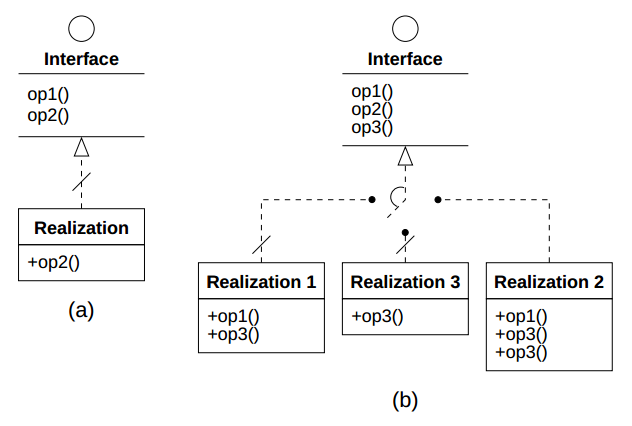
\includegraphics[width=7.5cm]{figuras/inflated_interface}
    \caption{Exemplos de uso de interfaces infladas \cite{guto_thesis}.}
\end{figure}


%%%%%


\section{Modos de Compilação}

Para compilar o EPOS, usa-se a ferramenta \verb+make+, através de um conjunto de \verb+makefiles+. As configurações referêntes à compilação podem ser encontradas no arquivo \verb+makedefs+, onde pode-se mudar o \emph{cross compiler} a ser usado, o modo de compilação (que será descrito a seguir), e arquitetura desejada.

%3 types of modes

O EPOS pode ser compilado de três formas diferentes:

\begin{description}
\item[Library] O sistema é compilado junto com a aplicação, sem distinção de espaço de endereçamento, existência de modo usuário nem chamadas de sistema.
\item[Builtin] Semelhante ao \emph{library}, com a diferença de que o SO é colocado nos endereços mais altos, e a aplicação nos endereços mais baixos (mas ainda usam o mesmo espaço de endereçamento), em contraste ao \emph{library} que mistura os dois. O principal uso desse modo é para depuração e desenvolvimento\cite{EPOS}.
\item[Kernel] Existe dois espaços de endereçamento diferentes, com modo usuário e kernel, com uma interface de chamada de sistema entre eles. Existe o conceito de \emph{task}.

\end{description}

%tools

Durante o processo de compilação do EPOS, duas ferramentas próprias são chamadas: \verb=eposcc= e \verb=eposmkbi=. O \verb=eposcc= é uma \emph{script} auxiliar do processo de compilação, é nela em que é diferenciado o modo de compilação do EPOS, e é nele que é acertada a ordem de ligação (\emph{linkage}) dos construtores globais do EPOS, algo muito importante para a inicialização do SO, como é descrito na seção \ref{sec:inicializacao}.
Já o \verb=eposmkbi= é uma ferramenta cujo objetivo é criar uma imagem ``bootável'' do SO com a aplicação. Esta imagem é uma imagem de virtualização de disco, com as metainformações necessárias já adicionadas à ela \cite{tarcisio}. Estas metainformações são adicionadas também à \verb=struct= \verb+System_info+, para que seja posteriormente usada pelo EPOS durante sua inicialização.



\section{Inicialização}
\label{sec:inicializacao}
O EPOS inicia executando um conjunto de códigos escritos em assembly, chamados de crts.
No crt, a primeira tarefa feita na inicialização do EPOS é a configuração das pilhas do sistema. Feito isto, o EPOS trata de limpar a seção .bss, para futuro reuso.
Antes de ser chamado o construtor dos demais objetos globais, a UART e Display são inicializados, assim é possível mais facilmente depurar o código dos construtores.
Então o EPOS começa a chamar o construtor global de cada componente do sistema. O crt consegue localizar onde está localizado cada construtor devido à forma como o EPOS foi compilado e ligado (\emph{linked}). A figura \ref{fig:initialization} ilustra num diagrama de sequência a ordem de construção dos objetos globais.

\fig{0.58}{initialization}{Diagrama de sequência da inicialização do EPOS}

Primeiro é construído o \verb+First_Object+, cuja principal função é apenas ser um ponto de entrada conhecido para o primeiro objeto do sistema.
Em seguida, é construído \verb+Init_System+. É neste construtor que todos os mediadores de hardware são construídos, com exceção da UART que já foi previamente construída no crt. Neste construtor, primeiramente é inicializado o \emph{timer}, MMU, e, se disponível, o TSC (\emph{Time Stamp Counter}). Em seguida o construtor aloca uma porção de memória para futuro uso da heap do sistema. Feito isto, o SCU (\emph{Snoop Control Unit}), tratador de interrupções e alarme são também construídos.

\verb+Init_Application+ é responsável por alocar a heap da aplicação, através da requisição de páginas da MMU. \verb+Init_First+ chama o inicializador das \emph{threads}, que então inicializa a \emph{thread} da aplicação e a \emph{idle thread}, que é uma \emph{thread} especial que é executada quando o escalonador não encontra outra \emph{thread} pronta para executar. Em seguida à criação destas \emph{threads}, é chamado \verb+context->load()+ da \emph{thread} da aplicação, fazendo com que o fluxo de execução seja finalmente transferido para a aplicação.

\section{Traits}
\label{sec:traits}
Existem 4 arquivos traits.h que devem ser levados em consideração em um porte, dois deles devem ser completamente reescritos. Os arquivos \verb+./include/traits.h+ e \verb+/include/system/traits.h+ (onde `.' é a pasta raiz do código) possuem configurações gerais do EPOS, que, a princípio, devem ser independentes de arquitetura. Na prática há alguns pequenos ajustes que devem ser feitos nesses arquivos, pois é lá que se define, por exemplo, se o EPOS trabalhará em um processador \emph{multicore}, se utilizará \emph{scratchpad}, quais componentes estarão em modo de depuração e etc; entretanto isto se resume a trocar o valor de algumas variáveis de \emph{true} para \emph{false} e vice-versa.

Os outros dois arquivos são \verb+./include/mach/zynq/traits.h+ e\\ \verb+./include/arch/armv7/traits.h+. Essa divisão é necessária pois, como dito anteriormente, é possível de um mesmo processador estar em diferentes \emph{machines}, e, caso seja necessário fazer um porte para aquela plataforma, bastaria modificar os arquivos da pasta \emph{mach}, deixando os da pasta \emph{arch} praticamente intactos, o que facilita muito novos portes.

O arquivo \verb+./include/arch/armv7/traits.h+ trata das opções específicas do processador, portanto é lá que opções como \emph{endianess}, velocidade de \emph{clock}, número de \emph{cores}, tamanho da \emph{heap} e \emph{stacks}, bem como outras opções pertinentes ao mapeamento de memória e opções da MMU podem ser configuradas.

No arquivo de traits da \emph{machine}, ficam as opções de configuração de componentes como a UART, controlador de interrupções, \emph{timer}, e qualquer componente de interfaceamento externo à placa (rede, por exemplo). Componentes podem ser facilmente ativados ou desativados nestas opções.

\section{Interrupções}


Como o EPOS foca do desempenho da aplicação, em seu design opta-se por utilizar a menor quantidade possível de interrupções, e evitá-las sempre que possível, isto contribui também para que o sistema seja mais previsível. Se a aplicação não precisar de componentes específicos que necessitem interrupções (como um rádio, por exemplo), a única interrupção a ser tratada será a do \emph{timer}, já que o escalonador e alarm necessitam dele.

%interrupções (indexação de um vetor de interrupções pelo seu ID)
%exception -> ic_handler -> timer_handler -> alarm handler
%                                         -> scheduelr handler

A sequência de chamadas de função, dado o recebimento de uma interrupção de \emph{timer} está ilutrada na figura \ref{fig:exception_handling}. Exception é um código em assembly cujo objetivo é salvar o contexto no recebimento da chamada, chamar o tratador de interrupções padrão, e restaurar o contexto após isto. O tratador de interrupções do \emph{interrupt controller} (IC) possui um vetor de tratadores de interrupção, onde para cada número de interrupção, há uma entrada correspondente no vetor. Este tratador então lê o registrador responsável por armazenar o número da interrupção gerada (esta parte é dependente de arquitetura, na Zedboard uma interrupção de timer tem número 29, por exemplo), indexa seu vetor e chama o tratador apropriado. Chegando no tratador do \emph{timer}, este chama os tratadores de todos os componentes que dependem de um \emph{timer}, neste caso o \verb+Alarm+ e \verb+Scheduler+.

\fig{0.18}{exception_handling}{Sequência de chamada de tratadores de interrupção. A interrupção gerada neste exemplo foi uma de \emph{timer}}. 



\section{Gerenciamento de Memória}
\label{sec:gerenciamento}
Uma das principais funções de um sistema operacional é o gerenciamento de memória. Isto inclui organizar a memória (mapeamento de memória, definição do que cada região da memória guarda, etc) e gerenciamento (manter registro de páginas livres, definir permissões, etc).

% MMU::alloc

Para entendermos como isto é feito, primeiro é necessário entendermos como funciona a abstração da MMU no EPOS. Isto se dá com 4 classes principais, a \verb+ARMv7_MMU+, que possui a lista de memória livre, a \verb+Page_Table+, que mapeia porções de até 1MB de endereço virtual para físico, \verb+Chunk+, que nada mais é que um conjunto de \verb+Page_Tables+, e, finalmente, \verb+Directory+, que é um conjunto de \verb+Chunks+ (ou \verb+Page_Tables+).

A classe \verb+ARMv7_MMU+ possui uma uma lista de porções de memória livre, gerenciadas pelas funções \verb+alloc+ e \verb+free+. A granularidade destas porções de memória é a de um \emph{frames}
\footnote{Frame é uma porção de tamanho fixo de memória física (normalmente 4KB). A diferença entre uma página e um frame é que um frame referece à uma porção da memória física, enquanto uma página referece à uma porção de memória virtual.}.
Note que esta lista utiliza os endereços \textbf{físicos} destas porções de memória.

A tabela de páginas da MMU do ARMv7, assim como a do IA32, possui dois níveis. Na nomenclatura da ARM, a tabela de nível mais alto é a tabela L1 (de \emph{level}), onde cada entrada desta tabela aponta para outra tabela (uma tabela L2).
Cada entrada da tabela L2 possui o endereço físico correspondente ao endereço virtual requisistado. A maneira como esta tabela é usada para traduzir um endereço virtual para um físico varia de arquitetura para arquitetura, sendo esta parte explicada detalhadamente na seção \ref{sec:mmu}.

Nas abstrações do EPOS, a classe que gerencia a tabela L2 é a \verb+Page_Table+, e a classe que gerencia a tabela L1 é a \verb+Directory+. Portanto uma \verb+Page_Table+ é apenas um vetor, onde em cada posição está escrita uma posição de memória física, junto de algumas \emph{flags} (que definem permissões, ``cacheabilidade'' e etc). O número máximo de entradas numa \verb+Page_Table+ é dependente de arquitetura. No ARMv7 são 256 entradas de 4 bytes (mapeando até 1MB de memória portanto), e no IA32 são 1024 entradas (que mapeiam até 4MB).

\verb+Chunk+ é uma classe bastante importante, e, apesar de simples, é importante que se tenha um bom entendimento sobre como ela funciona.
Cria-se um chunk para alocar uma certa porção de memória, em um espaço de endereçamento próprio. 

Esta classe recebe dois parâmetros: A quantidade de bytes a serem alocados, e as \emph{flags} a serem usadas. \verb+Chunk+ então calcula quantas tabelas de páginas serão necessárias para mapear a quantidade de bytes requisitada, e então cria estas páginas contiguamente (em qualquer lugar da memória, a ser decidido pela função \verb+alloc+).

\verb+Chunk+ então chama a função \verb+map+ de \verb+Page_Table+ para mapear aquela porção da memória. Cada \emph{frame} é requisitado pela função \verb+alloc+, o que significa que cada \verb+Page_Table+ pode estar apontando para qualquer posição da memória, não estando os \emph{frames} necessariamente contiguos na memória física, apesar que eles serão \textbf{contíguos} no espaço de memória virtual mapeada num mesmo \verb+Chunk+.

Portanto esta classe efetivamente aloca uma porção de memória em um espaço de endereçamento próprio, este fato será bastante importante quando discutirmos a criação das heaps de usuário e do sistema.

%Directory

Já a classe directory é responsável por gerenciar e unificar todas estas porções de memória. Sua principal função é a \verb+attach+, que tomando como parâmetro um \verb+Chunk+, mapeia cada uma de suas páginas contiguamente (isto é, cria uma entrada em directory que a aponta para uma página criada em \verb+Chunk+, para cada página).

A figura \ref{fig:mmu_translation} ilustra a interação entre os conteúdos das entradas de \verb+Directory+ e \verb+Page_Table+ com a memória física. A quantidade de bits usada para indexar as tabelas é dependente de arquitetura. Aqui, os primeiros 12 bits indexam a tabela de \verb+Directory+, os 8 bits seguintes indexam a tabela de \verb+Page_Table+, e os últimos 12 bits são simplesmente copiados do endereço virtual para o físico. Mais detalhes sobre este processo na seção \ref{sec:mmu}, em particular na imagem \ref{fig:translation}.

%\fig{0.42}{mmu_translation}{Interação entre \verb+Directory+ e \verb+Page_Table+ com a memória física.}


\fig{0.45}{mmu_translation}{Interação entre Directory e Page\_Table com a memória física. Neste exemplo, o endereço virtual 0xAB2FF123 seria traduzido para o endereço físico 0xDEAD1123. A última posição de memória física indexável neste exemplo é 0x1FFFF\_\_\_ pois a Zedboard dispõe de 512MB.}

\verb+Directory+ não sabe a qual \verb+Chunk+ uma determinada \verb+Page_Table+ pertence, e a tradução de endereços pode ocorrer independente desta informação. Na figura \ref{fig:mmu} é ilustrada a interação entre as classes discutidas.

\fig{0.20}{mmu}{Diagrama de classes da MMU.}


%make a diagram showing how MMU alloc a physical page, and how the heap lends pages that were already allocated in the MMU's point of view.

\subsection{Heaps}

A heap é responsável por armazenar e gerenciar os dados dinâmicos criados durante a execução da aplicação (a cada \verb+malloc/new+ executado, por exemplo). Existe duas heaps: A do sistema, e a do usuário. É possível compilar o EPOS com apenas a heap do sistema, quando o desenvolvedor decide que a aplicação deverá rodar em modo privilegiado, não sendo usado portanto o modo usuário (isto é configurável nos \verb+traits+).

A memória da heap é alocada através de um \verb+Chunk+. É neste ponto que pode-se atribuir flags que limitam as permições de acesso (a heap de usuário é alocada sem restrições de acesso, já a do sistema aloca uma porção de memória que só pode ser acessada em modo privilegiado). É por usar um \verb+Chunk+ também que do ponto de vista da aplicação, é como se ela tivesse acesso à todo o espaço de memória. Note que do ponto de vista da MMU (e sua lista de memória livre), é como se a porção de memória da heap estivesse em uso, já a heap vê sua porção de memória como livre.

A heap trabalhada com uma lista de memória livre (igual à da MMU), só que ao contrário da MMU, que aloca somente páginas (frames) inteiras de memória, a heap aloca quantidades de memória com a granularidade de bytes.

Para que a heap do sistema e a heap do usuário seja corretamente usada, faz-se no EPOS \emph{overload} do operador \verb+new+ e \verb+delete+, e \emph{placement new}. Por exemplo, um \verb+new A()+ chamaria a seguinte sequencia de funções:

\begin{lstlisting}
inline void * operator new(size_t bytes) {
    return malloc(bytes);
}
inline void * malloc(size_t bytes) {
    if(Traits<System>::multiheap)
        return Application::_heap->alloc(bytes);
    else
        return System::_heap->alloc(bytes);
}
\end{lstlisting}

O compilador se encarrega de avaliar o \verb+sizeof+ de \verb+A+, e envia como parâmetro para o operador \verb+new+. \verb+multiheap+ é um atributo dos traits que define se o sistema possui uma heap de usuário separada da do sistema ou se é usada somente uma única heap.

Para o sistema alocar memória usando sua própria heap com o operador \verb+new+, faz-se um \emph{overload} do \emph{placement new}, como segue:

\begin{lstlisting}
enum System_Allocator {SYSTEM};

inline void * operator new(size_t bytes, const EPOS::System_Allocator & allocator) {
    return EPOS::System::_heap->alloc(bytes);
}
\end{lstlisting}

Feito isto, para alocar, dentro do EPOS, alguma porção de memória utilizando o operador \verb+new+ com a heap do sistema, basta escrever \verb+(SYSTEM)+ logo após o \verb+new+, por exemplo:

\begin{lstlisting}
_timer = new (SYSTEM) Alarm_Timer(handler);
\end{lstlisting}


\section{Escalonadores}

%falar dos escalonadores que o EPOS suporta
%falar do gio <3

O EPOS suporta diversos escalonadores, desde os de propósito geral até escalonadores de tempo real \emph{multicore}.
Do primeiro tipo, temos o \emph{Round Robin} e \emph{First-Come, First-Served}, do segundo, \emph{Rate Monotonic}, \emph{Deadline Monotonic} e \emph{Earliest Deadline First} (global, particionado e agrupado), e também o escalonador descrito em \cite{gio}.

\fig{0.30}{edf_uml}{Diagrama de classes para os escalonadores que usam a política \emph{Earliest Dealine First} \cite[p.~184]{gio}.}

O EPOS é projetado de modo a permitir grande reuso ao se escrever um escalonador. Por exemplo, há três escalonadores que utilizam a política EDF (\emph{Earliest Deadline First}), que nada mais é que um critério de escolha de \emph{thread}, onde neste caso procura-se escolher aquela cujo \emph{dealine} está mais próximo, por isto separou-se esta parte das especificidades que existem entre os escalonadores. 

A figura \ref{fig:edf_uml} ilustra a relação entre as classes dos escalonadores que herdam de EDF.  Não é o objetivo deste trabalho entrar em detalhe nas especificidades dos diferentes escalonadores do EPOS, entretanto será colocada uma breve descrição destes três escalonadores EDF para que a figura fique clara.

\begin{description}

\item[PEDF:] O \emph{partitioned} EDF (particionado) possui uma fila de tarefas a serem escalonadas para cada processador. A escolha de que fila cada tarefa é atribuida é feita de forma estática. Cada tarefa executa sempre no mesmo processador, não havendo migração destas. 

\item[GEDF:] O EDF global utiliza uma única fila de tarefas, e atribui uma tarefa toda vez que um processador fica livre. A vantagem deste escalonador sobre o PEDF é que ele consegue escalonar conjuntos de tarefas que o PDF não conseguiria, entretanto seu desempenho costuma ser menor e menos previsível, pois migrar uma tarefa de um processador para o outro é custoso, e gera um mal aproveitamento das memórias \emph{cache}.

\item[CEDF:] Este é o caso geral do PEDF e GEDF. Neste escalonador há uma fila para cada grupo de processadores (\emph{cluster}). Por exemplo, numa arquitetura que usa 8 processadores, poder-se-ia fazer 4 grupos de 2 processadores cada, totalizando 4 filas. Somente há migração de tarefas entre processadores de um mesmo grupo. Caso o grupo seja do tamanho do número de cores, tem-se o GEDF, e se cada grupo tiver apenas um processador, obtem-se o PEDF.

\end{description}




















\chapter{Implementação dos Mediadores de Hardware}

% Eu poderia descrever como eu tenho que incluir cada classe feita em ./include/system/types.h, opções de traits, etc..

Nesta seção será discutido como foi o porte de cada mediador de hardware, explicando as decisões tomadas.

A grosso modo, o processo de inicialização do sistema envolve \cite[p.~110]{ug585.1.7}:

% Fazer imagem BONITA sobre a table abaixo

\begin{enumerate}
	\item Definir a tabela de vetores.
	\item Invalidar \emph{caches}, TLB, \emph{branch predictor}
	\item Preparar tabelas de tradução de página.
	\item Configurar as pilhas dos diferentes modos de execução.
	\item Carregar o endereço base da tabela de páginas no registrador apropriado para ser usado pela MMU.
	\item Ativar a MMU.
	\item Ativar a L2, ativar a L1.
	\item Pular para o ponto de entrada a aplicação.
\end{enumerate}

Estes e outros passos (como inicialização do GIC) são explicados em detalhe nas seções que seguem.


\section{Mediador da UART}

A inicialização da UART foi feita de acordo com o sugerido pelo manual em \cite[p.~554]{ug585}. Nesta seção será comentado as decisões tomadas na configuração inicial da UART, em particular por causa dos momentos em que o manual exigia que o desenvolvedor tomasse uma decisão.

A primeira decisão que foi necessária é a de escabelecer qual será a taxa de transmissão (\emph{Baud Rate}) da UART. 

\begin{figure}[ht!]
    \centering
    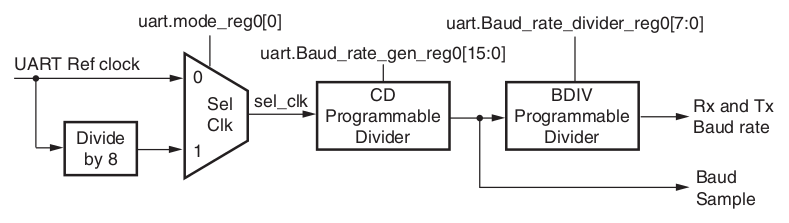
\includegraphics[width=10cm]{figuras/uart_board_rate}
    \caption{Esquemático de como é criada a taxa de transmissão.}
	\label{fig:uart}
\end{figure}

Primeiramente foi necessário configurar o \emph{clock} de referência da UART. Para isto, deve-se dividir o \emph{clock} que vem do I/O PLL (que por sua vez deriva do PS\_CLK, que é o \emph{clock} geral do sistema). Recomenda-se dividir o \emph{clock} da I/O PLL de modo a se obter 50 ou 33 MHz.
O \emph{clock} da I/O PLL, por padrão, multiplica o PS\_CLK (de 33.33 MHz) por 26, resultando num \emph{clock} de 866 MHz.
No manual diversas vezes é usado como exemplo para o \emph{clock} de referência (que é mostrado sob o nome de \verb+UART Ref clock+ na figura \ref{fig:uart}) da UART como 50 MHz, portanto, arbitrariamente, escolheu-se esse valor. Logo, deve-se configurar o registrador UART\_CLK\_CTRL, responsável por configurar o \emph{clock} de entrada da UART, para dividir este \emph{clock} vindo da I/O PLL por 17 ($866/17 = 50$).

Agora, com este \emph{clock} estabelecido, que vamos chamar de sel\_clk (de acordo com a nomenclatura do manual), devemos calcular quanto será a taxa de transmissão.
Após alguma pesquisa em fóruns de desenvolvedores de software básico, foi observado que uma taxa de transmissão de 9600 bps é bastante comum, portanto, assumindo este valor, a próxima etapa é configurar os dois divisores de \emph{clock} que ajustam a taxa de transmissão, como indicado na figura \ref{fig:uart}.

O primeiro divisor chama-se CD (\emph{clock divider}), que configura a constante para se dividir o \emph{clock}, e BDIV um segundo divisor usado para sobreamostragem, organizado como mostrado na figura \ref{fig:uart}. O valor da taxa de transmissão final é calculado da seguinte forma:
\begin{equation}
	\text{taxa de transmissão} = \frac{sel\_clk}{CD \times (BDIV+1)}
\end{equation}

O valor padrão de BDIV é 15, portanto, fixando-se este valor e resolvendo a equação por CD, temos que $CD = 325$. Configurando-se estes valores nos seus respectivos registradores, obtém-se a taxa de transmissão desejada de 9600 bps.

Após estas configurações, dentre outras que o manual descreve, a UART está pronta para ser usada. Os dois principais métodos usados da UART são o \verb+put+ e o \verb+get+, o primeiro escreve um caractere na saída serial, sendo que este pode ser lido, por exemplo através de uma entrada USB, para imprimir estes caracteres numa tela; algo muito útil para depuração.


\section{Mediador do \emph{Timer}}

Um \emph{timer} permite contar um certo número de ciclos, e, ao final da contagem, ele emite uma interrupção ao GIC, para que então o processador trate este evento. Entretanto note que é possível de existir mais \emph{timers} sendo usados logicamente do que \emph{timers} físicos disponíveis, significando que um mesmo \emph{timer} deve conseguir servir a mais de uma requisição simultaneamente.

Portanto não podemos apenas configurar um \emph{timer} para contar initerruptamente até passar o tempo que desejamos, do contrário novas requisições sobreescreveriam a anterior. Para ilustrar, suponha que se queira contar por 10 segundos, como o \emph{clock} do \emph{timer} é de 333 MHz (periodo $\frac{1}{333 \times 10^6}$s), bastaria configurar o \emph{timer} para contar por $10 \times 333 \times 10^6$ ciclos e então chamar o \emph{handler} associado à interrupção gerada quando o \emph{timer} chegar em zero.

Agora imagine que, no cenário acima, enquanto o \emph{timer} ainda está servido àquela solicitação de contagem, apareça outra solicitação, de um alarme por exemplo, e queria contar por 20 segundos. Se esta solicitação sobrescrever o registrador de configuração do \emph{timer}, a solicitação anterior não terá seu pedido atendido a tempo. Note também que o escalonador de processos também estará usando este \emph{timer}.

Para resolver este problema, na arquitetura do EPOS existe o conceito de ticks (algo parecido com o que se faz no Linux), onde se configura um \emph{timer} para gerar interrupções em um intervalo regular, intervalo este que deve ser pequeno o suficiente para poder atender a demanda de contagens de pequenos valores, assim como não ser pequeno demais ao ponto de gastar mais processamento tratando as interrupções geradas pelo \emph{timer} do que servindo à outras funções. Assim, cada objeto que instancia (ou usa) um \emph{timer}, como o Alarm, Scheduler e Chronometer, nunca realmente tocam em algum registrador do \emph{timer} (portanto esses componentes são independentes de arquitetura), e, no lugar disso, computam quantos ticks, isto é, quantas interrupções de \emph{timer} aconteceram.

Para exemplificar o funcionamento destes componentes, tomemos o escalonador de processos. No construtor do escalonador, é enviado como parâmetro o periodo de escalonamento, ou seja, quanto tempo (no máximo) uma \emph{thread} pode executar antes de ser escalonada. Para se saber quantos ticks devem ser contados antes de se escalonar um processo, basta dividir a frequência em que os ticks incrementam, pela frequência de escalonamento. Por exemplo, se o \emph{timer} gera uma interrupção a cada 1 milisegundo (1000 Hz), e o escalonador escalona um processo a cada 10 milisegundos (100 Hz), o número de ticks a se contar é $1000/100 = 10$ ticks. Estes são os valores usados na implementação também.

No caso do Alarm em específico, internamente há uma fila com todas as requisições de alarme, ordenado do menor tick ao maior. Quando ocorre uma interrupção de \emph{timer}, é chamado primeiramente o \emph{handler} que gerencia esta fila, e, caso um alarme desta fila já tenha esperado os ticks que requisitou, então o \emph{handler} desse alarme é chamado (este \emph{handler} é definido pelo usuário que instanciou o alarme).


O construtor do \verb+Zynq_Timer+ recebe como parâmetro a frequência que o contador deve contar, assim como o \emph{handler} que deve ser chamado quando esta contagem terminar (isto é, a função chamada quando acontecer uma interrupção devido ao \emph{timer} ter chego a zero), e um número chamado \verb+channel+, que serve para demultiplexar qual \emph{handler} deve ser chamado.

A classe \verb+Zynq_Timer+ possui um atributo estático (e portanto único para todas as instâncias) definido como \verb+Zynq_Timer*+ \verb+_channels[CHANNELS]+, onde \verb+CHANNELS+ é uma constante com o número de diferentes classes usando o \emph{timer} (Scheduler e Alarm). Este vetor é necessário pois, quando uma interrupção de \emph{timer} acontece e o \emph{handler} do \emph{timer} é chamado, este \emph{handler} pode iterar sobre ele, chamando todos os respectivos \emph{handlers} daquelas classes. Abaixo segue um exemplo de código de como isto pode ser feito:


\label{int_handler}
\begin{lstlisting}
Zynq_Timer * Zynq_Timer::_channels[CHANNELS];

void Zynq_Timer::int_handler(IC::Interrupt_Id id)
{
  if((!Traits<System>::multicore ||
    (Traits<System>::multicore && (Machine::cpu_id() == 0)))
    && _channels[ALARM])
  {
    _channels[ALARM]->_handler();
  }

  if(_channels[SCHEDULER] &&
    (--_channels[SCHEDULER]->_current[Machine::cpu_id()] <= 0))
  {
    _channels[SCHEDULER]->_current[Machine::cpu_id()] =
      _channels[SCHEDULER]->_initial;
    _channels[SCHEDULER]->_handler();
  }
}
\end{lstlisting}

No código, \verb+_current+ guarda o número de ticks atual daquele \emph{timer} (para cada processador), e \verb+_initial+ guarda o número inicial de ticks que foi configurado na inicialização do do escalonador. Note então que a cada interrupção de \emph{timer}, o tratador do alarme será chamado (no caso do primeiro processador), já o do escalonador, somente a cada certo número de ticks ele será chamado (cerca de 100 na implementação).

Os 4 principais registradores a se trabalhar para configurar o \emph{timer} são o \verb+load+, registrador onde se escreve por quantos ciclos se deve contar; o \verb+counter+, que é o registrador que contém o atual valor contado, sendo decrementado a cada ciclo até chegar em zero, chegando em zero o é gerada uma interrupção número 29; registrador \verb+control+, que permite configurar certos comportamentos do \emph{timer}, como o de ativa-lo, ativar modo cíclico, ativar interrupções e atribuir um valor para o \verb+prescale+; e finalmente o registrador \verb+interrupt status+, que, como o nome indica, permite que se leia o status das interrupções de timer. Todos os timers trabalham à metade do \emph{clock} do sistema, ou seja, usando o \emph{clock} CPU\_3x2x.

Durante a inicialização do sistema, o \emph{timer} é configurado para gerar interrupções periodicamente, e esta configuração não é alterada durante a execução da aplicação. Como o construtor do \verb+Zynq_Timer+ recebe uma frequência como parâmetro, é necessário se converter esta frequência para um número de ciclos a se contar. Para isto, é necessário se levar em conta a frequência com que o contador é decrementado, para então se definir um valor a ser decrementado periodicamente de modo a fornecer a frequência desejada.

Como sabemos que o \emph{clock} ao qual o \emph{timer} está submetido é metade do \emph{clock} do sistema, e que antes dele chegar ao contador, este mesmo \emph{clock} é dividido por um divisor chamado \verb+prescaler+ (que divide pelo valor configurado nele mais 1), podemos dizer a frequência F\_dec de decremento do contador é de:
\begin{equation}
	\text{F\_dec} = \frac{\text{CPU\_6x4x}}{2 \times (PRESCALER+1)}
\end{equation}
Logo, usando a mesma linha de racioncínio exposta no exemplo de cálculo de ticks, temos que o valor a ser carregado no \verb+load_register+ (que será chamado de \verb+load_value+), sendo F a frequência que se deseja configurar o \emph{timer}, é:
\begin{equation}
	\text{load\_value} = \frac{\text{CPU\_6x4x}}{2 \times (PRESCALER+1) \times F}
\end{equation}
Ou de maneira mais simples:
\begin{equation}
	\text{load\_value} = \frac{\text{F\_dec}}{F}
\end{equation}
Precisamos agora definir o \verb+prescaler+. Definimos ele como a razão entre o \emph{clock} do sistema pela frequência desejada ($\text{prescaler}=\frac{\text{clock}}{2 \times F}$). Há a premissa de que a frequência desejada não será maior que a do \emph{clock} do \emph{timer}, pois é impossível contar mais rápido que isto. Normalmente esta razão ($\frac{\text{clock}}{2 \times F}$) será um número maior que 255, já que o clock costuma ser muito mais rápido, e como o campo onde se registra o valor do prescaler possui apenas 8 bits, frequentemente o prescaler será 255.


\section{Mapeamento de Memória}

Por padrão, as 8 primeiras palavras da memória (ou seja, os primeiros $8 \times 4 = 32$ bytes) devem possuir instruções específicas. A primeira palavra (memória posição 0) contém a primeira instrução a ser executada, e, nas 7 palavras seguintes, fica a tabela de vetores (\emph{vector table}). Como abaixo da instrução inicial há uma tabela que não se deseja executar no momento de inicialização do sistema, esta primeira instrução necessariamente é um \emph{jump} para uma outra região, para aí então se iniciar o processo de \emph{boot}. 
As demais 7 palavras, pertencentes à tabela de vetores possuem, similarmente, \emph{jumps} para o código onde o tratador da exceção se localiza. A primeira instrução da tabela (posição 0x4) deve conter um \emph{jump} o tratador de uma exceção do tipo undefined instruction, depois, nas próximas palavras, a software interruption, prefectch abort, data abort, reserved, irq e, finalmente, fiq, nesta ordem. Vide seções \ref{sec:interrupt} e \ref{sec:operating_modes} para mais detalhes.


%desmontamento do binário da imagem do EPOS
Desmontando-se o binário da imagem produzida na compilação do EPOS (\emph{dump}), deve-se obter uma saída semelhante a esta exemplificada abaixo em seus primeiros 32 bytes:

\label{dump}
\hspace*{-1cm}\vbox{
\begin{verbatim}
00000000 <_vector_table>:
	 0:  ldr	pc, [pc, #2044]	; 804 <_start_addr>
	 4:  ldr	pc, [pc, #2044]	; 808 <_undefined_instruction_addr>
	 8:  ldr	pc, [pc, #2044]	; 80c <_software_interrupt_addr>
	 c:  ldr	pc, [pc, #2044]	; 810 <_prefetch_abort_addr>
	10:  ldr	pc, [pc, #2044]	; 814 <_data_abort_addr>
	14:	 ldr	pc, [pc, #2044]	; 818 <_reserved_addr>
	18:  ldr	pc, [pc, #2044]	; 81c <_irq_handler_addr>
	1c:  ldr	pc, [pc, #2044]	; 820 <_fiq_handler_addr>
\end{verbatim}
}

Também foi necessário definir as pilhas (\emph{stacks}) do sistema, assim como reservar um espaço para a pilha dos tratadores de interrupção. O \emph{layout} escolhido segue na tabela \ref{tab:stacks}.
Este é o \emph{layout} usado durante o desenvolvimento. Somente as pilhas de usuário e de algum modo privilegiado (como o supervisor) são necessárias, portanto a pilha de supervisor acabaria por englobar as demais posições que aparecem na tabela \ref{tab:stacks}. Na próxima seção é explicado como foi feito para não precisar reservar espaço na memória para as demais pilhas.

\begin{table}[hb]
	\centering
	\begin{tabular}{ccc}
		\hline \hline
		Pilha & Endereço base & Tamanho máximo (bytes)\\[0.5ex]
		\hline
		Supervisor (CPU1)		& \verb+0x00080000+ & 500784\\
		Supervisor (CPU0)		& \verb+0x00100000+ & 524288\\
		Irq						& \verb+0x00100040+ & 64\\
		System					& \verb+0x00100080+ & 64\\
		Abort					& \verb+0x001000c0+ & 64\\
		Fiq						& \verb+0x00100100+ & 64\\
		Undefined				& \verb+0x00100140+ & 64\\[1ex]
		\hline
	\end{tabular}
	\caption{Pilhas do sistema com seus tamanhos e posições.}
	\label{tab:stacks}
\end{table}

Lembrando que pilhas, num sistema operacional, tradicionalmente crescem em direção à posições menores da memória, por isto que, por exemplo, a pilha Irq possui 64 bytes, já que $\texttt{0x100040}-\texttt{0x100000} = 40_{16} = 64_{10}$. A pilha do usuário, portanto, localiza-se na última posição da memória (512 MB neste caso) e cresce para ``baixo'' (posições menores de memória) a partir de lá.


A tabela \ref{tab:mem} ilustra o restante do mapeamento de memória feito. APP\_DATA é a posição onde será armazenado a seção de dados do EPOS, sendo que 1KB é seguramente mais do que o suficiente para esta seção. É possível descobrir qual é o tamanho da seção de dados em um binário através do comando \verb+size <binary>+. Com este comando, observou-se que, na atual versão do EPOS, a seção de dados possui 436 bytes, e a .bss 188 bytes.

System Info é uma \verb+struct+ que guarda informações sobre o SO, que é usado durante a inicialização do sistema (e pode ser descartado mais tarde).

Para a MMU, é necessário 3600 KBs para mapear todo o espaço de endereçamento virtual (vide a seção \ref{init_pages} para entender porque apenas 3600 KBs); a tabela e páginas usada pela MMU está indicada como ``Tabela MMU'' na tabela \ref{tab:mem}.
``Livre'' indica memória não usada. Esta porção não pode ser alocada pois a tabela da MMU precisa iniciar numa posição de memória alinhada à 16 KB.

SYS\_HEAP é a \emph{heap} do sistema operacional. Note que as pilhas das \emph{threads} ficam dentro da \emph{heap} do sistema, por isto ele deve ter um tamanho adequado para poder alocar memória suficiente para o número de \emph{threads} que espera-se executar.
% APP\_STACK é a pilha da aplicação; note que esta pilha cresce em direção contrária a da \emph{heap}, portanto um excesso de uso da \emph{heap} ou da pilha pode acabar corrompendo a memória da aplicação, gerando um erro que são chamados em alguns sistemas operacionais de \emph{stack overflow}.




\begin{table}[ht]
	\centering
	\begin{tabular}{ccc}
		\hline \hline
		Dado & Endereço base & Tamanho Alocado\\[0.5ex]
		\hline
		APP\_DATA		& \verb+0x00100140+ & 1KB\\
		System Info		& \verb+0x00100540+ & 260 bytes\\
		Livre			& \verb+0x00100644+ & ~14KB\\
		Tabela MMU		& \verb+0x00104000+ & 3600KB\\
		SYS\_HEAP		& \verb+0x00488000+ & 128MB\\[1ex]
%		APP\_STACK		& \verb+0x1ffffffc+ & \~380MB
		\hline
	\end{tabular}
	\caption{Mapeamento de memória.}
	\label{tab:mem}
\end{table}


\section{Porte do Controlador de Interrupções}

Para se usar o controlador de interrupções (que será referenciado como GIC no restante desta seção, de \emph{Generic Interrupt Controller}), é necessário antes inicializar o distribuidor de interrupções e as interfaces dos processadores.

É no distribuidor que é determinada a prioridade de cada interrupção, e onde é decidido se determinada interrupção deve ou não ser encaminhada para a interface de um determinado processador. Todas as interrupções passam por ele.

A interface dos processadores é por onde os processadores se comunicam com o GIC. Nela o processador pode confirmar que recebeu a interrupção (\emph{acknowledge}), indicar que terminou de tratar a mesma, definir prioridades entre diferentes interrupções, indicar uma política de preempção de interrupções, ou mesmo desligar esta interface. Como o GIC é dividido logicamente é ilutrado na imagem \ref{img:gic}.

\begin{figure}[ht!]
    \centering
    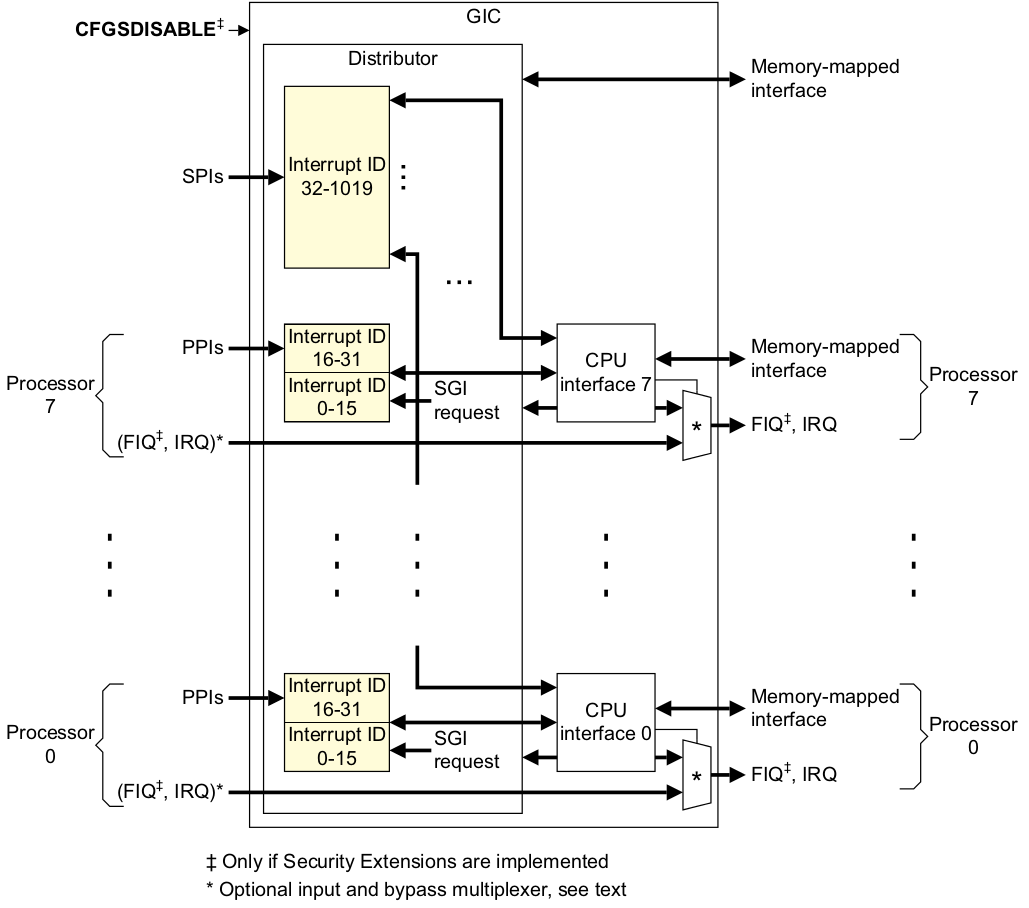
\includegraphics[width=9.5cm]{figuras/gic}
    \caption{Divisão lógica do GIC.}
    \label{img:gic}
\end{figure}

\subsection{Inicialização}

Na inicialização do distribuidor, através dos registradores mapeados em memória de configuração do mesmo, é definido, para cada uma das possíveis interrupções, se elas são \emph{level-sensitive} ou \emph{edge-triggered}.
Em seguida configura-se a prioridade de cada interrupção. A princípio todas as interrupções foram definidas como tendo a mesma prioridade, mas isto é configurável caso necessário.
É configurado então o processador-alvo de cada interrupção, isto é, para quais interfaces de processador uma determinada interrupção será encaminhada. Finalmente então são ativadas as interrupções \cite{gic}.

A inicialização da interface do processador é mais simples. Primeiro se configura a máscara de prioridade da CPU, isto é, qual é o nível de prioridade mínimo que uma interrupção precisa ter para interromper aquele processador. Na implementação, esta máscara está desativada. Depois configura-se a política de grupos de preempção. No GIC é possível separar interrupções em grupos de preempção, onde se define se determinado grupo pode preemptar determinado outro grupo. Todas as interrupções foram colocadas no mesmo grupo e interrupções podem ser preemptadas.

Adicionalmente a estas configurações, é possível de mascarar as interrupções FIQ e IRQ através do CPSR (\emph{Current Program Status Register}), alterando-se os bits 6 e 7 dele, para mascarar interrupções FIQ e IRQ, respectivamente. Normalmente é o que é feito quando é necessário mascaras as interrupções, enquanto se mantém as configurações do GIC.

\subsection{Fluxo de execução ao se receber uma interrupção}

O processador, ao receber uma interrupção, (portanto as interrupções estão ativas e não mascaradas pela interface ou pelo CPSR), para a execução do código que estava executando e então executa a instrução contida na tabela de vetores (mostrada na página \pageref{dump}) correspondente ao tipo de interrupção recebida. Esta instrução é um \emph{jump} para um tratador (\emph{handler}) daquele tipo de interrupção.

O principal tratador é o tratador de interrupções IRQ (\verb+irc_handler+), sendo que este precisa ser discutido com mais profundidade. Abaixo segue o código deste tratador:

\hspace*{-1cm}\vbox{
\begin{lstlisting}
43 void _irq_handler() {
44   ASMV(
45   // A few definitions
46   ".equ ARM_MODE_FIQ,      0x11 \n"
47   ".equ ARM_MODE_IRQ,      0x12 \n"
48   ".equ ARM_MODE_SVC,      0x13 \n"
49   ".equ IRQ_BIT,           0x80 \n"
50   ".equ FIQ_BIT,           0x40 \n"
51   // go to SVC
52   "msr cpsr_c, #ARM_MODE_SVC | IRQ_BIT | FIQ_BIT \n"
53   //save current context (lr, sp and spsr are banked registers)
54   "stmfd sp!, {r0-r3,r12,lr,pc}\n"
55 
56   "msr cpsr_c, #ARM_MODE_IRQ | IRQ_BIT | FIQ_BIT\n"//go to IRQ
57 
58   "sub r0, lr, #4 \n" // return from irq addr
59   "mrs r1, spsr   \n" // pass irq_spsr to svc r1
60   //go back to SVC
61   "msr cpsr_c, #ARM_MODE_SVC | IRQ_BIT | FIQ_BIT\n"
62   "add r2, sp, #24 \n" //sp+24 is the position of the saved pc
63   
64   // save return address into the pc position
65   "str r0, [r2] \n" 
66   "stmfd sp!, {r1} \n"   // save irq-spsr
67       
68   );
\end{lstlisting}
\begin{lstlisting}
71   IC::int_handler();
72     
73   ASMV(        
74   "ldmfd sp!, {r0}              \n"
75   "msr spsr_cfxs, r0\n"//restore IRQ's spsr value
76                        //to SVC's spsr             
77   "ldmfd sp!, {r0-r3,r12,lr,pc}^ \n" // restore context
78   //the ^ in the end of the above instruction makes the 
79   //spsr to be restored into svc_cpsr
80   );
81 }
\end{lstlisting}
}

Após selecionar qual handler chamar, o processador muda de modo, indo, no caso de uma interrupção IRQ, para o modo de execução IRQ. Neste modo há 3 registradores banqueados: O SPSR, que contém o valor do registrador CPSR imediatamente antes da interrupção, sendo necessário para que seja possível restaurar o valor original do CPSR após tratar a interupção; o LR (\emph{link register}), que contém o endereço da próxima instrução que seria executada imediatamente antes da interrupção mais 4; e, finalmente, o SP (\emph{stack pointer}), que aponta para a pilha própria desde modo (cada modo pode possuir sua própria pilha).

Para evitar desperdício de memória reservando uma pilha própria apenas para este modo, optou-se por não usar uma pilha no modo IRQ, e, no lugar disto, usar sempre a mesma pilha do modo supervisor (que é o modo de execução do processador quando ele inicia). Para isto, a primeira instrução a executar é uma mudança de modo para voltar ao modo supervisor, enquanto mantendo novas interrupções desligadas; lá é salvo o contexto na pilha daquele modo. Entretanto para que seja possível restaurar o fluxo de execução no mesmo estado em que o processador estava no momento imediatamente antes da interrupção, é necessário voltar ao modo IRQ para obter-se os valores contidos dos registradores banqueados SPSR e LR; após isto, pode-se então voltar ao modo \emph{supervisor}. Na linha 62 do código é somado 24 à pilha pois lá é a posição de memória onde está salvo o PC após ele ter sido empilhado na linha 54, e deseja-se sobreescrever aquele valor do PC pelo valor que estava contido no LR do modo IRQ (menos 4), pois aquela é a próxima instrução que seria executada antes da interrupção. Feito isto, salva-se o valor do SPSR do modo IRQ no topo da pilha (que é o valor do CPSR pré-interrupção), para ser restaurado ao CPSR mais tarde.

Agora que o contexto foi salvo corretamente para ser restaurado, pode-se então chamar um tratador de interrupções genérico (que será discutido mais a frente) e escrito em C++. Após o \verb+int_handler+ da linha 71 retornar, é feita a restauração do contexto. Primeiro se salva o CPSR salvo na pilha no SPSR, na última instrução (\verb+ldmfd+), na forma em que ela está (com um \^{} no final dela e com o PC na lista), ela automaticamente restaurará o valor que está no SPSR para o CPSR. Como o PC está na lista, o fluxo de execução terá retornado a executar as instruções de antes da interrupção ocorrer.

Agora será discutido como que as interrupções são tratadas individualmente. O corpo do \verb+int_handler+ é bastante curto, então vale a pena escreve-lo aqui:

\begin{lstlisting}
void Zynq_IC::int_handler()
{	
    unsigned int icciar_value = CPU::in32(IC::GIC_PROC_INTERFACE 
        | IC::ICCIAR);
    IC::Interrupt_Id id = icciar_value & IC::INTERRUPT_MASK;

    if(id == 1023){
        kout << "Spurious interruption received\n";
        return;
    }
    _vector[id](id);
    CPU::out32(IC::GIC_PROC_INTERFACE | IC::ICCEOI, icciar_value);
}
\end{lstlisting}

A primeira coisa que o tratador faz e descobrir qual é o número da interrupção que foi gerada, para assim saber como tratar aquela interrupção. Isto é feito lendo-se o registrador ICCIAR (\emph{Interrupt Acknowledge Register}), que provê o número da interrupção e também o processador endereçado.
É possível que uma interrupção já tenha sido tratada por outro processador, quando isto acontece, o GIC emite uma \emph{Spurious Interruption} para indicar isto. Quando se detecta isto, o tratador não precisa tomar nenhuma outra ação, basta retornar a execução normal.

Com o número da interrupção em mãos, pode-se então chamar o tratador daquele tipo de interrupção. O \verb+_vector+ é um vetor de \emph{handlers}, onde para cada posição $i$, existe o tratador da interrupção número $i$. Para sinalizar que uma interrupção foi tratada, deve-se escrever no registrador ICCEOI (\emph{End of Interruption}) o número lido no ICCIAR (ou seja, o número da interrupção e processador de destino).


Normalmente, interrupções de \emph{timer} são o tipo mais frequente de interrupção durante a execução do sistema. Dele dependem o escalonador de processos (ou \emph{threads}), Delay, Chronometer e Alarm. Como mencionado na seção do porte do \emph{timer}, uma mesma interrupção pode gerar a chamada de mais de um handler, como a do \emph{timer} que chama a do Alarm e do escalonador. Com isto fica ilustrado que uma única interrupção pode gerar a chamada de vários tratadores para esta mesma interrupção.


\section{MMU}
\label{sec:mmu}
%nice image in p.87 ug585

%na inicialização, é liberada toda a memória, colocando ela numa lista
%MMU é inteiramente controlada pelo coprocessador CP15
%http://www.slideshare.net/prabindh/enabling-two-level-translation-tables-in-armv7-mmu
%http://www.embedded-bits.co.uk/2011/mmucode/
%http://lxr.free-electrons.com/source/arch/arm/mm/proc-v7-2level.S?a=arm



As principais funções de uma MMU (\emph{Memory Managemend Unit}) são proteção de memória, ou seja, não permitir acesso a certas regiões da memória por processos não autorizados, e de fazer o mapeamento de memória virtual para memória física, mapeamento este que facilita a escrita de aplicações já que o desenvolvedor dela não precisará estar ciente de como a memória é mapeada internamente pelo sistema operacional.

A MMU consegue cumprir estes dois objetivos (e outros mais) através do uso de uma tabela de tradução de páginas (que chamaremos de TTP), onde, a grosso modo, cada linha desta tabela é indexada pelo valor do endereço virtual, e na entrada correspondente há o endereço físico assim como \emph{flags} que indicam, dentre outras coisas, se aquela região pode ou não ser acessada pela aplicação em execução.

Esta tabela é salva na memória principal (RAM) do sistema, e configurar a MMU significa especialmente criar métodos para gerenciar e popular esta tabela. Para entender como isto é feito, será explicado agora como é estruturada esta tabela, como que ocorre a tradução de memória virtual para física, e o que cada entrada da tabela deve ter.

\subsection{Estrutura da Tabela de Tradução de Página}

A TTP possui dois níveis, portanto, desconsiderando-se a TLB, é necessário dois acessos à TTP para traduzir um endereço, caso configurado para páginas de 4 KB. a MMU suporta páginas de 4 KB e 64 KB, assim como seções de 1 MB e 16 MB. Como cada endereço virtual corresponde à exatamente uma entrada na TTP, usar páginas grandes reduz o tamanho da TTP (consequentemente o uso de memória por ela), entretanto usar páginas menores (4 KB) melhoram muito a eficiência da alocação dinâmica de memória e desfragmentação \cite[p.~77]{ug585.1.7}, porém mapear um espaço de 4 GB exigiria milhões de entradas na tabela. Foi justamente para conciliar estes fatores, que decidiu-se por uma tabela de dois níveis, como será melhor ilustrado a seguir.

A tabela de tradução páginas nível um (TTP1), também chamada de ``\emph{master table}'', divide todo o espaço de endereçamento de 4 GB em 4096 seções de 1 MB, portanto, como cada entrada desta tabela tem o tamanho de uma palavra, seu tamanho total em memória é de $4 \times 4096 = 16$ KB. Os 2 bits menos significativos (lsb) de cada entrada desta tabela, definem que tipo de entrada ela é, que pode ser um dos 5 tipos:

\begin{itemize}
	\item Bits lsb 00: É uma ``fault entry'', e gera uma exceção do tipo \emph{prefetch} ou \emph{data abort}, dependendo do tipo de acesso. Este tipo de entrada indica que não há mapeamento virtual para esta região.
	\item Bits lsb 01: Indica a posição de memória de uma tabela de páginas (nível 2).
	\item Bits lsb 10 com bit 18 em 0: Aponta para uma seção de 1 MB.
	\item Bits lsb 10 com bit 18 em 1: Indica uma seção de 16 MB, este tipo de entrada exige 16 posições na TTP1.
	\item Bits lsb 11: Reservado, gera faltas de tradução e não deve ser usado.
\end{itemize}

A figura \ref{fig:l1_entry} ilustra o formato de uma entrada da TTP1. NS significa \emph{non-secure}, e só tem semântica com extensões de segurança habilitadas (fora do escopo do trabalho). SBZ significa \emph{should be zero}. Bits C, B, TEX e AP serão explicados após a explicação do formato de uma entrada da TTP2, pois esta tem campos análogos.

\begin{figure}[hb!]
    \centering
    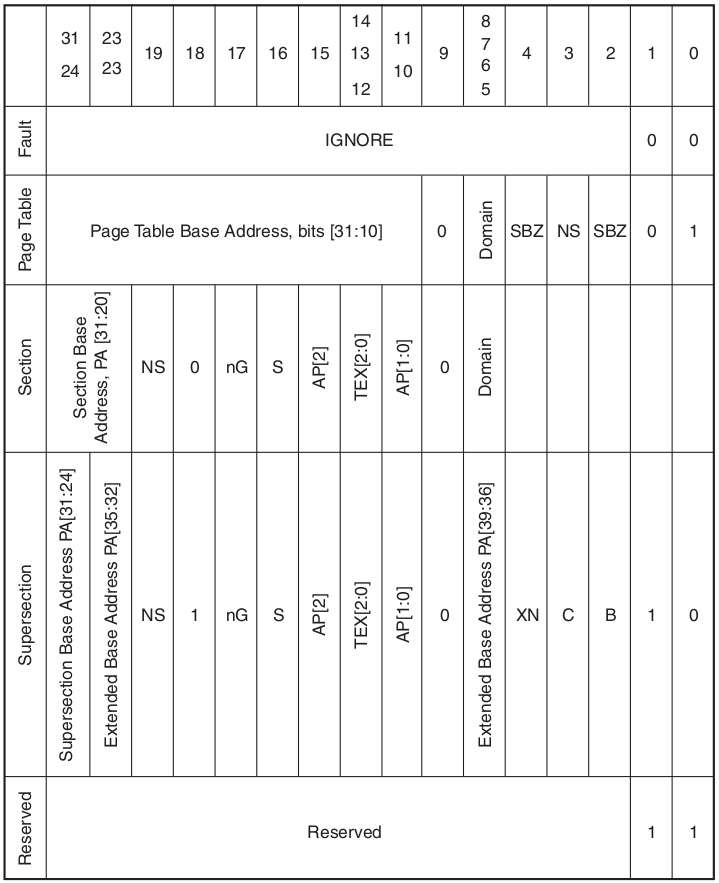
\includegraphics[width=9cm]{figuras/l1_entry}
    \caption{Formato de uma entrada da tabela de tradução de páginas nível 1.}
	\label{fig:l1_entry}
\end{figure}

Vamos agora entender como se traduz de um endereço virtual, o endereço de uma TTP2. No coprocessador CP15, existe um registrador chamado TTBR (dois na realidade, TTBR0 e TTBR1), sigla de \emph{Translate Table Base Register}, onde é guardado o endereço da primeira posição da TTP1. Com a MMU ligada, quando há um acesso à memória, automaticamente a MMU pulará para a posição indicada no TTBR, e indexará esta tabela usando os 12 bits mais significativos do endereço virtual. A maneira exata de como é feito este cálculo é mostrada na figura \ref{fig:translation}.

Na posição de memória encontrada no passo anterior, estará uma entrada da TTP1 no formato indicado na figura \ref{fig:l1_entry}. No caso de uma entrada que indica uma outra TTP, os primeiros 22 bits indicam o endereço onde estará esta tabela, com os demais bits em 0, com exceção do último e os do campo de domínio (que será explicado a seguir). Com estas informações, a MMU já pode localizar a posição da TTP2. Para saber qual das entradas da TTP2 deve ser selecionada, é usado os bits [19:12] do endereço virtual para indexar a TTP2.

Os 4 bits do campo de domínio indicam em qual dos possíveis 16 domínios de memória aquela região se encontra, um domínio é apenas um conjunto de regiões de memória. A utilidade disto é que se pode, para cada domínio, especificar como será o controle de acesso nele. Cada domínio pode estar configurado (pelo registrador DACR) como um dos três tipos de acesso: \emph{Acesso não permitido}, qualquer acesso a esta região gera uma falta de domínio; \emph{Cliente}, permissões de acesso são verificadas, e podem gerar uma falta de permissão; e \emph{Administradores}, onde permissões de acesso não são verificadas (bits AP e APx são ignorados).

\begin{figure}[h]
    \centering
    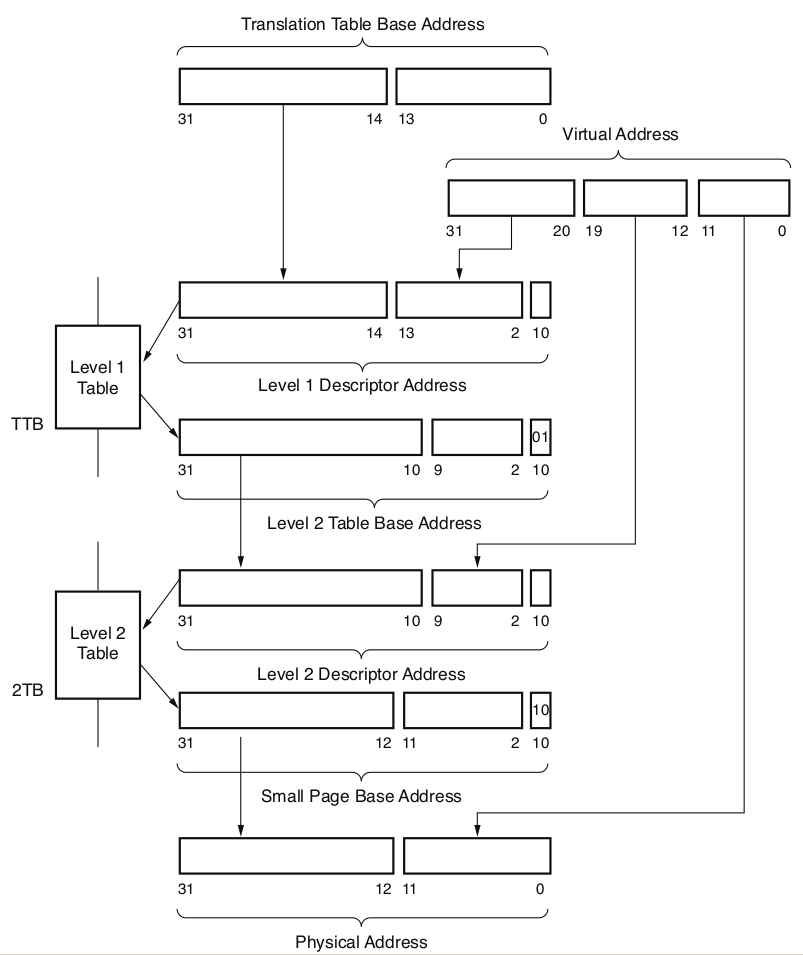
\includegraphics[width=9cm]{figuras/translation}
    \caption{Processo de tradução de memória virtual para física.}
    \label{fig:translation}
\end{figure}

A TTP2 possui 256 entradas, cada uma com o tamanho de uma palavra, logo, cada TTP2 precisa de 1 KB de memória. Note que como uma entrada da TTP1 provê 22 bits para endereçar uma TTP2, esta TTP2 pode efetivamente estar localizada em qualquer região da memória, já que 22 bits são suficientes para indexar qualquer região de 1 KB de memória.

A figura \ref{fig:l2_entry} ilustra como é o formato de uma entrada na TTP2. Os 2 bits menos significativos indicam se a página possui 4 KB, 16 KB ou se a região não está mapeada. Com o endereço de uma entrada da TTP2 em mãos, basta combinar os 20 bits mais significativos desta entrada com os 12 bits menos significativos do endereço virtual, e teremos traduzido o endereço virtual para um físico.

\begin{figure}[h]
    \centering
    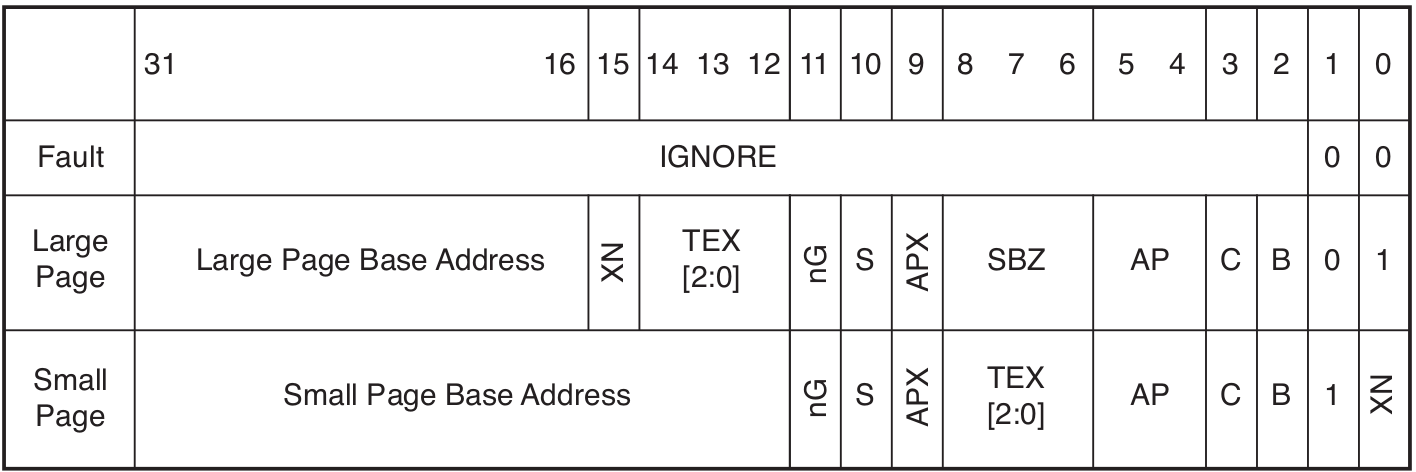
\includegraphics[width=9cm]{figuras/l2_entry}
    \caption{Processo de tradução de memória virtual para física.}
    \label{fig:l2_entry}
\end{figure}

Agora vamos discutir o que cada campo de uma entrada da TTP2 significa.

\textbf{AP e APx:} São os bits que codificam o tipo de acesso que aquela porção de memória possui. Estes bits só são checados caso do domínio seja de \emph{Cliente}. Um acesso que não possui as permissões necessárias geram uma exceção do tipo \emph{prefetch} ou \emph{data abort}. APx e AP[2] são sinônimos. A tabela \ref{tab:apx} ilustra os diferentes tipos de acesso que podem ser codificados.

\begin{table}[h]
	\centering
	\begin{tabular}{ccccc}
		\hline \hline
		APx & AP[1] & AP[0] & Privilegiado & Não Privilegiado\\[0.5ex]
		\hline
		0 & 0 & 0 & Sem acesso & Sem acesso\\
		0 & 0 & 1 & Escrita/Leitura & Sem acesso\\
		0 & 1 & 0 & Escrita/Leitura & Sem acesso\\
		0 & 1 & 1 & Escrita/Leitura & Sem acesso\\
		1 & 0 & 0 & \~{} 			& \~{}		 \\
		1 & 0 & 1 & Leitura 		& Sem acesso \\
		1 & 1 & 0 & Leitura 		& Leitura	 \\
		1 & 1 & 1 & \~{} 			& \~{}		 \\[1ex]
		\hline
	\end{tabular}
	\caption{Codificações das permissões de acesso.}
	\label{tab:apx}
\end{table}


\textbf{TEX:} Controla políticas de compartilhamento de memória, caso aquela região seja compartilhada.
\textbf{C e B:} Estes campos combinados controlam a política de ``cacheamento'' daquela região de memória, ou seja, se ela pode ser salva na cache, e se pode, qual o algoritmo a a ser usado, como \emph{write-back} ou \emph{write-though}, e também políticas de \emph{write-allocate}.
\textbf{S:} Bit que determina que aquela porção de memória é compartilhada entre processadores.
\textbf{nG:} Responsável pela proteção de memória intraprocessos. Uma região marcada como não global (nG = 1) tem associado à ela um número que o SO atribui a cada processo. Isto permite que a TLP possa ter diferentes mapeamentos simultaneamente sem necessidade de substituir uma entrada.
\textbf{xN:} Bit que marca a região como não executável. É importante por questões de segurança, já que o \emph{fetch} especulativo de instruções pode ler uma porção de memória que possui dados sensíveis.


\subsection{Inicializando a Tabela de Páginas}
\label{init_pages}
Agora que sabemos como as TTPs são estruturadas, bem como o formato de cada entrada dela, podemos finalmente popular esta tabela. Há várias estratégias para fazer isto \cite{mmutheory}, dependendo da forma desejada de mapeamento, por exemplo:

\begin{itemize}
	\item Mapeamento por Demanda: Pode-se fazer com que determinado endereço virtual não possua um mapeamento correspondente a priori, gerando uma exceção que é tratada criando-se uma TTP2 que mapeie aquela área.
	\item Mapeamento 1 para N: Com o advento do bit nG, é possível também mapear uma mesma área de memória virtual em diferentes áreas da memória física, de modo que quando o escalonador de processos escalona num novo processo (ou \emph{thread}), ele também modifica o mapeamento de memória, deste modo, diferentes processos poderiam usar uma mesma determinada posição de memória virtual.
	\item Mapeamento 1 para 1: É o mapeamento mais simples possível, de modo que a posição de memória virtual X corresponde a posição de memória física X.
\end{itemize}

%Mapeamento adotado:

No mapeamento adodotado, a princípio mapeia-se em em uma relação 1:1 os primeiros 512MB de memória virtual para os 512MB de memória física disponíveis, ou seja, o endereço virtual será o mesmo que o endereço físico. Entretanto note que com o uso de \verb+Chunks+ e \verb+Address_space+ é possível alocar uma porção de memória em um mapeamento próprio, como explicado na seção \ref{sec:gerenciamento}.

Suponha que a MMU esteja ativa, e deseja-se salvar determinada informação numa determinada posição de memória física P, cujo endereço virtual correspondente seja V. Se apontarmos um ponteiro para a posição P, e escrever nesta posição, a MMU automaticamente irá interpretar P como sendo memória virtual, e irá traduzir P para uma outra posição de memória física qualquer e imprevisível.

Agora suponha que o mapeamento de memória esteja dividido no meio, de tal modo que a segunda metade faz uma relação 1:1 com a memória física. Deste modo, dado um endereço físico P, é possível calcular qual é seu endereço virtual V. 

No EPOS foi feito um mapeamento semelhante, o intervalo de memória virtual [0x20000000 : 0x3FFFFFFF] mapeia para [0x0 : 0x1FFFFFFF]. Portanto \verb+P | 0x20000000 == V+, onde | é o operador \emph{or} de bits. Veja o seguinte exemplo de código:

\begin{lstlisting}
static Log_Addr phy2log(Phy_Addr phy){
    return phy | PHY_MEM;
}
static Phy_Addr calloc(unsigned int frames = 1) {
    Phy_Addr phy = alloc(frames);
    memset(phy2log(phy), 0, sizeof(Frame) * frames);
    return phy;
}
\end{lstlisting}

\fig{0.6}{memory_map}{Mapeamento de memória adotado. Os primeiros 512MB de memória virtual são mapeados 1:1 para a memória física, enquanto os 512MB de memória virtual seguintes mapeiam para os os mesmos 512MB de memória física. De 1GB à 4GB é um mapeamento simples 1:1, referentes aos registradores mapeados em memória.}

\verb+memset+ irá tentar escrever no endereço enviado como parâmetro, que será interpretado como um endereço virtual, que então será traduzido para um físico correspondente. Entretanto no lugar de um endereço físico, é enviado o endereço lógico no lugar, para que este seja então traduzido para o endereço físico que desejamos. Esta é uma maneira do SO internamente burlar a tradução da MMU.

O restante da memória virtual (1GB-4GB) é traduzido numa relação 1:1. Esta região de memória corresponde principalmente a registradores mapeados em memória, não sendo, portanto, memória RAM. A figura \ref{fig:memory_map} ilustra o mapeamento adotado.

Note que num mapeamento completo 1:1, a TTP1 tomaria $4\times4096$ bytes (4KB), e as 4096 TTP2 (uma para cada posição da TTP1) tomariam $4\times256\times4096$ bytes (4MB). Entretanto como o mapeamento virtual do intervalo 512MB-1GB pode usar as mesmas tabelas TTP2 que foram criadas com o mapeamento do intervalo 0-512MB, pode-se economizar $4\times256\times512$ bytes. Portanto, no total, as tabelas de tradução de páginas usadas pela MMU usam 3600KB de memória RAM.

%Realização deste mapeamento no código:

Em um mapeamento 1 para 1, para popular as TTPs, primeiramente, em um loop, itera-se 512 vezes (já que há 512 de RAM), salvando em posições sucessivas de uma determinada região da memória os endereços das TTP2s, levando-se em conta as \emph{flags} acima mencionadas, após as 512 posições, itera-se pelas por mais 512 posições, mapeando novamente os primeiros 512 MB de memória física. Após isto, mapeia-se as posições restantes em relação 1:1. Feito isto, é necessário também popular cada TTP2 que foi apontada na TTP1, em um processo semelhante. Em um mapeamento por demanda, marca-se as regiões da memória virtual como não mapeadas, com a diferença que, ao invés de apenas abortar o acesso, cria-se dinamicamente aquele mapeamento.

Após feita as tabelas, a MMU está pronta para ser ativada. A MMU é controlada pelo coprocessador CP15, é nele que são guardados os registradores de configuração, endereço base para a TTP, dentre outras funções. Escrevendo-se 1 no bit menos significativo no registrador c1 (SCTLR) deste coprocessador, a MMU é ativada.


\section{Mediador da CPU}

O mediador da CPU encapsula uma série de funções/rotinas usadas pelo sistema. A maior parte destas funções precisam ser escritas diretamente em assembly, ou usam informações dependente de arquitetura. Este mediador não precisa ser instanciado nem inicializado, ele é apenas um conjunto de funções necessárias por outros componentes.

Entre as funções deste mediador estão:

\begin{itemize}

\item Ativar/desativar máscara de interrupções de um dado processador.
\item Rotinas para desligar, suspender e reiniciar o sistema.
\item Função usada pelo escalonador para fazer a troca de contexto.
\item Salvar/alterar registrador que guarda o endereço base da tabela de páginas.
\item Funções primitivas usadas em semáforos e mutexes, como tsl (\emph{test and set lock}), finc e fdec.
\item Inicializar CPU 1.
\item Funções para escrita/leitura de registradores.

\end{itemize}


Nesta classe também há uma classe interna chamada \verb+Context+. Ela possui funções para salvar e carregar o contexto do processador, e atributos para salvar cada registrador de propósito geral da arquitetura (incluindo sp e pc e cpsr). Esta classe é usada no momento da criação de uma \emph{thread}, e durante a troca de contexto.



\section{Mediador SCU}

\section{Multicore}

Ao se ligar a placa, apenas a CPU0 executa código, e é função dela fazer as inicializações necessárias para então ligar o segundo processador (CPU1). Inicialmente, a CPU1 executa uma instrução (\verb+wfe+) que o coloca em modo de espera por evento (\emph{Wait for Event Mode}). Para sair deste modo, a CPU0 precisa emitir uma instrução do tipo evento de sistema, \verb+sev+ (\emph{System Event}). Quando a CPU1 recebe este sinal, ele imediatamente executa a instrução que está no endereço 0xfffffff0, localização onde a CPU0 deve previamente ter escrito uma instrução que faça a CPU1 fazer um \verb+jump+ para o ponto de entrada do que se deseja executar com a CPU1. Note que a posição 0xfffffff0 é uma região reservada da memória, e não corresponde à uma posição da RAM (é o mesmo princípio de registradores mapeados em memória).

Isto é suficiente para fazer o segundo processador passar a executar código, entretanto esta é a parte simples, ter dois processadores rodando tem várias implicações sobre como deve ser o \emph{design} de cada componente do sistema, pois agora há a preocupação com coerência e consistência de memória, condições de corrida {\emph{racing conditions}) e etc.

Um exemplo de componente que deve que ser adaptado para levar em conta que há mais de um processador, está no código da página \pageref{int_handler}, pois apenas o CPU0 pode escalonar processos no \emph{design} escolhido. Também é necessário levar em conta o fato de que agora é necessário invalidar a cache privada da CPU1 também, assim como ativar seu\emph{timer} privado. Através do coprocessador que controla a MMU, é possível de configurar políticas de coerência de memória, como citado na seção \ref{sec:mmu}.




\chapter{Conclusão}

%Falar dos algoritmos de escalonadores já implementados no EPOS, e que agora eles podem rodar no multicore implementado (preferencialmente teste isso, please)

%Fale de trabalhos futuros na conclusão! Frisar bastante os trabalhos que podem ser construídos em cima do porte, como o quadcoptero e a tese do Giovani.

Este trabalho visou descrever como foi feito o porte do sistema operacional EPOS para a Zedboard. Foram explicadas as decisões de projeto feitas, de modo que as próximas pessoas que venham a portar o EPOS para outra arquitetura, possam entender o raciocínio por trás do que foi implementado, para que o que foi aqui exposto possa ser adaptado a outros contextos.

Foi necessário explicar uma série de especificidades da arquitetura para expor como que é feito o interfaceamento do software com o hardware, e como um sistema operacional pode controlar e configurar componentes de hardware.

Este porte possibilitou novos cenários de aplicação do EPOS, espera-se portanto que isto contribua para estimular novas linhas de pesquisa com este sistema operacional na arquitetura trabalhada.




\bibliographystyle{ufscThesis/ufsc-alf}
\bibliography{references}

%--------------------------------------------------------
% Elementos pós-textuais
%\apendice
%\chapter{Exemplificando um Apêndice}
%Texto do Apêndice aqui. 

\anexo
\chapter{Artigo}
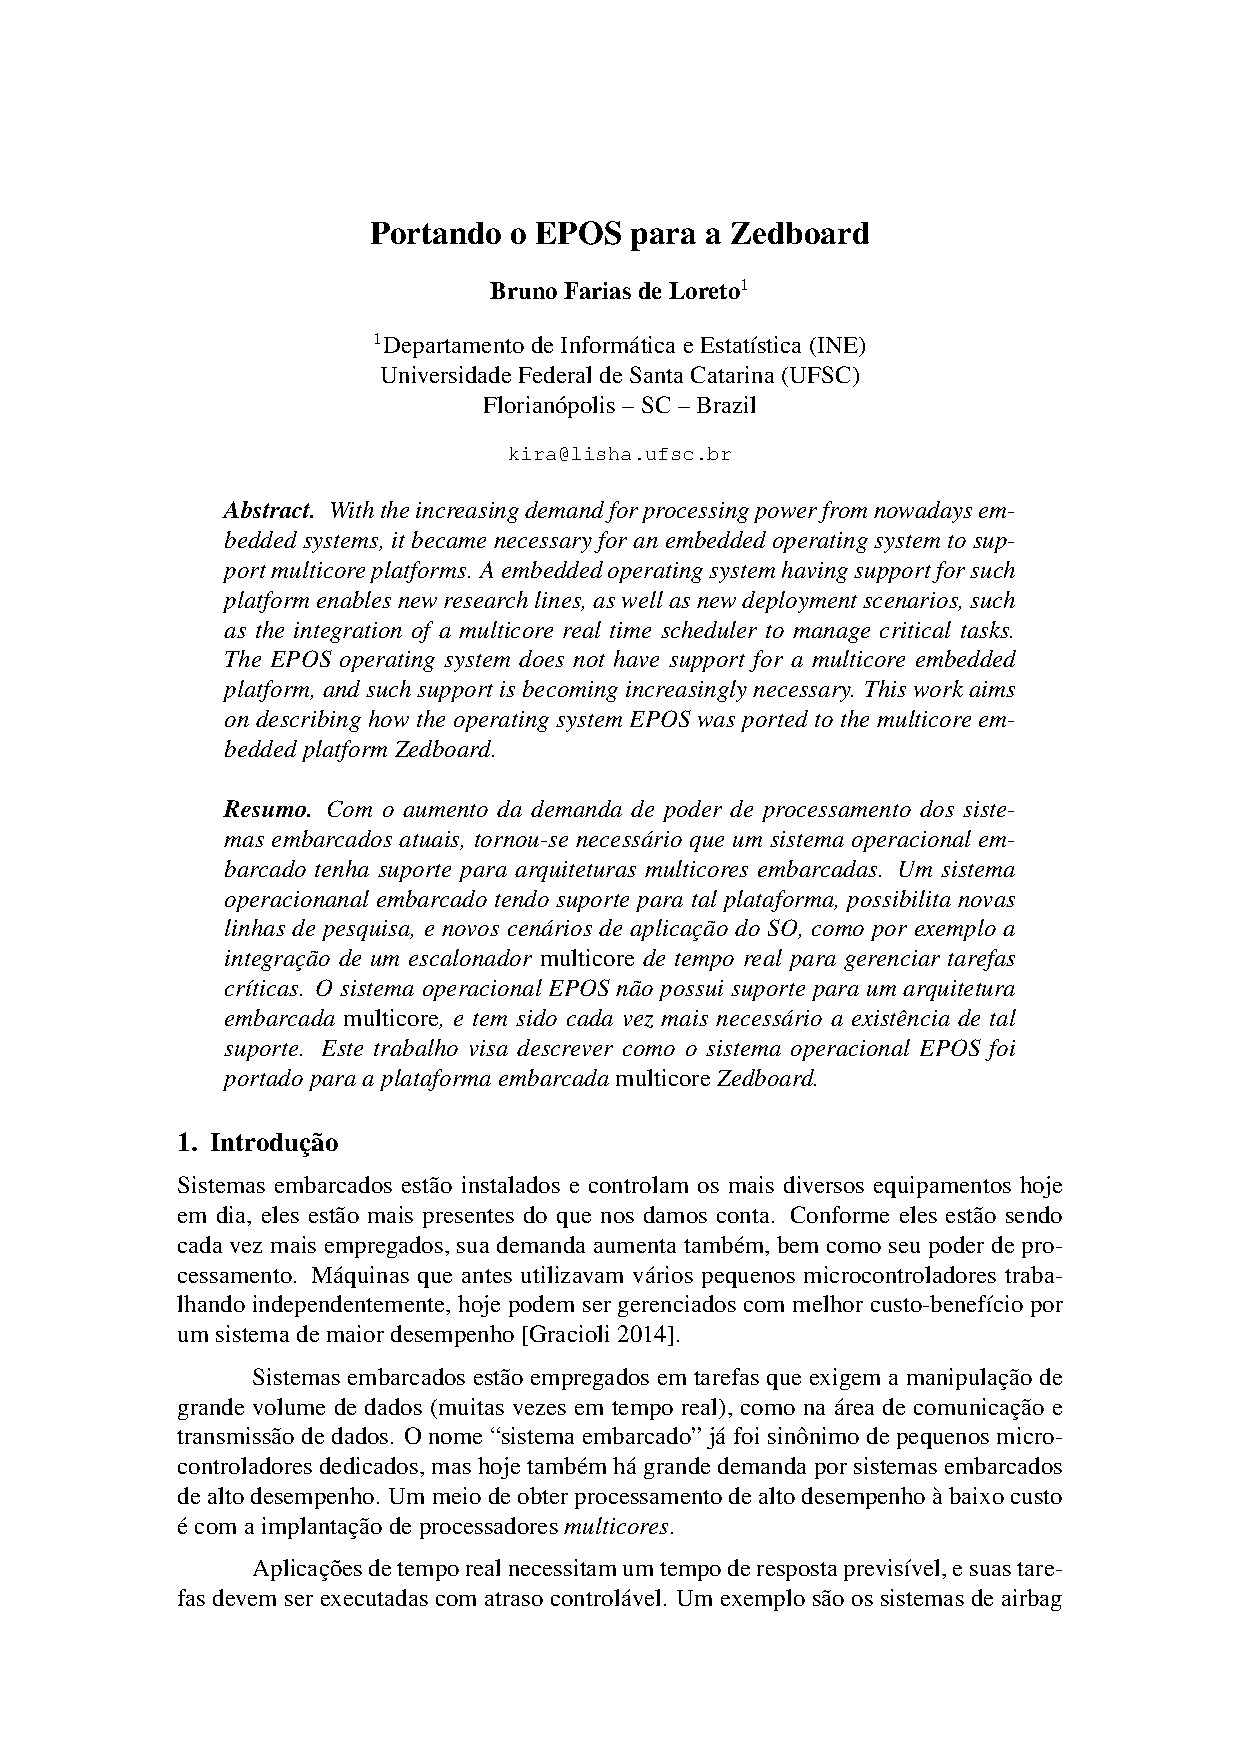
\includepdf[pages={1-18}]{artigo.pdf}
\chapter{Códigos Fonte}
Como este trabalho se trata de um acrescimo de suporte à um sistema operacional, seria inviável colocar todos os códigos fonte neste apêndice. No lugar disto, foi colocado as principais classes implementadas. Note que há outros arquivos que necessitaram modificação que não estão expostos aqui.

\section{cpu.h}
\input{fontes/cpu.h}

\section{cpu.cc}
\input{fontes/cpu.cc}

\section{cpu\_init.cc}
\input{fontes/cpu_init.cc}
%%%
\section{mmu.h}
\input{fontes/mmu.h}

\section{mmu.cc}
\input{fontes/mmu.cc}

\section{mmu\_init.cc}
\input{fontes/mmu_init.cc}
%%%
\section{ic.h}
\input{fontes/ic.h}

\section{ic.cc}
\input{fontes/ic.cc}

\section{ic\_init.cc}
\input{fontes/ic_init.cc}
%%%
\section{uart.h}
\input{fontes/uart.h}
%%%
\section{timer.h}
\input{fontes/timer.h}

\section{timer.cc}
\input{fontes/timer.cc}

\section{timer\_init.cc}
\input{fontes/timer_init.cc}


\end{document}
